% This file was converted to LaTeX by Writer2LaTeX ver. 1.9.3
% see http://writer2latex.sourceforge.net for more info
\documentclass[a4paper]{article}
\usepackage[utf8]{inputenc}
\usepackage{amsmath,amssymb,amsfonts,textcomp}
\usepackage[T1]{fontenc}
\usepackage[ngerman]{babel}
\usepackage{longfbox,fancyhdr}
\usepackage[margin=0.7874in,noheadfoot]{geometry}
\usepackage{hyperref}
\usepackage[pdftex]{graphicx}
% Outline numbering
\setcounter{secnumdepth}{0}
% Pages
\fancypagestyle{Standard}{\fancyhf{}
  \fancyhead[L]{}
  \fancyfoot[L]{}
  \renewcommand\headrulewidth{0pt}
  \renewcommand\footrulewidth{0pt}
  \renewcommand\thepage{\arabic{page}}
}
\pagestyle{Standard}
\begin{document}
\textbf{Prof. Dr. Maximilian Adler} [geb. 21.09.1884 in Budweis (Böhmen); gest. 16.10.1944 im KZ Auschwitz
(Generalgouvernement Polen)] war ein in wissenschaftlichen Kreisen anerkannter tschechoslowakischer Philologe und von
1932-1939 Professor für Klassische Philologie an der Karl-Ferdinands-Universität in Prag.

\begin{figure}[h]
\centering
\lfbox[margin-top=0.1181in,margin-right=0.1181in,margin-bottom=0.1181in,margin-left=0.1181in,border-style=none,padding=0mm,vertical-align=top,raise=-0.9055in]{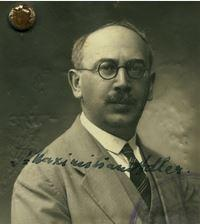
\includegraphics[width=1.5744in,height=1.7634in]{Kurzbiographien-img001.jpg}}
\end{figure}
Am 10.01.39 durch die tschechische Regierung, wegen seiner jüdischen Herkunft und seinem, den Nazianalsozialisten
missfallenden, starken Eintreten für den Zionismus, 'beurlaubt', wurde er schließlich am 06.03.1943 mit dem Transport
Cv in das Ghetto Theresienstadt deportiert. Dort leitete er das \textit{Bildungsreferat} und unterrichtete jüdische
Kinder. Er beteiligte sich an den kulturellen Aktivitäten im Ghetto und pflegte engen Umgang mit den anderen
prominenten Gefangenen, wie mit dem Rabbiner Leo Baeck, dem Psychiater Viktor Frankl und dem Geograf Alfred Philippson.
Im Propagandafilm ist er zu sehen in der Sequenz \textit{Vortrag} (33). Mit einem der letzten Transporte wurde er im
Oktober 1944 in das KZ Auschwitz gebracht und dort ermordet.


\bigskip

\textbf{Eigene Werke:}

\begin{itemize}
\item Quibus ex fontibus Plutarchus libellum ‚De facie in orbe lunae‘ hauserit. Wien 1910 (Dissertationes philologae
Vindobonenses 10,2)
\item Stoicorum veterum fragmenta. Vol. 4: Quo indices continentur. Leipzig 1924 
\item Studien zu Philon von Alexandreia. Breslau 1929
\end{itemize}

\bigskip

\textbf{Sekundärliteratur:}

\begin{itemize}
\item Susanne Blumesberger, Michael Doppelhofer, Gabriele Mauthe: Handbuch österreichischer Autorinnen und Autoren
jüdischer Herkunft 18. bis 20. Jahrhundert. Band 1: A–I. Hrsg. von der Österreichische Nationalbibliothek. Saur,
München 2002, ISBN 3-598-11545-8, S. 14.
\item Kulturní adresář ČSR.: Biografický slovník žijících kulturních pracovníků a pracovnic. 2. Ausgabe (1936), S. 10 
Miroslav Kárný: Terezínská pamětní kniha. Prag 1995, S. 1172  
\item Elena Makarova, Serge\u{\i} Makarov, Victor Kuperman: University over the abyss: the story behind 520 lecturers
and 2,430 lecturers in KZ Theresienstadt 1942–1944. Jerusalem 2000, S. 433  
\item Martin Sicherl: Erinnerungen an Prag (1933–1937). In: Eikasmós. Band 4, 1993, S. 85–94  Rudolf M. Wlaschek:
Biographia Judaica Bohemiae. Band 1 (2003), S. 4
\item 
\bigskip
\end{itemize}
\textbf{Internetquellen:}

\begin{itemize}
\item \url{https://yvng.yadvashem.org/nameDetails.html?itemId=1109013}
\item \url{https://www.holocaust.cz/de/opferdatenbank/opfer/74467-maximilian-adler/}
\item \url{https://de.wikipedia.org/wiki/Maximilian_Adler} 
\end{itemize}

\bigskip

\textbf{Bildquelle:}

\begin{itemize}
\item \url{https://www.holocaust.cz/de/opferdatenbank/opfer/74467-maximilian-adler/}
\end{itemize}
\textbf{Karel Ančerl} (urspr. Antscherl) [geb. 11.04.1908 in Tučapy (Österreich-Ungarn); gest. 03.07.1973 in Toronto
(Kanada)] war ein tschechoslowakischer Dirigent.

\begin{figure}[h]
\centering
\lfbox[margin-top=0.1181in,margin-right=0.1181in,margin-bottom=0.1181in,margin-left=0.1181in,border-style=none,padding=0mm,vertical-align=top,raise=-0.9055in]{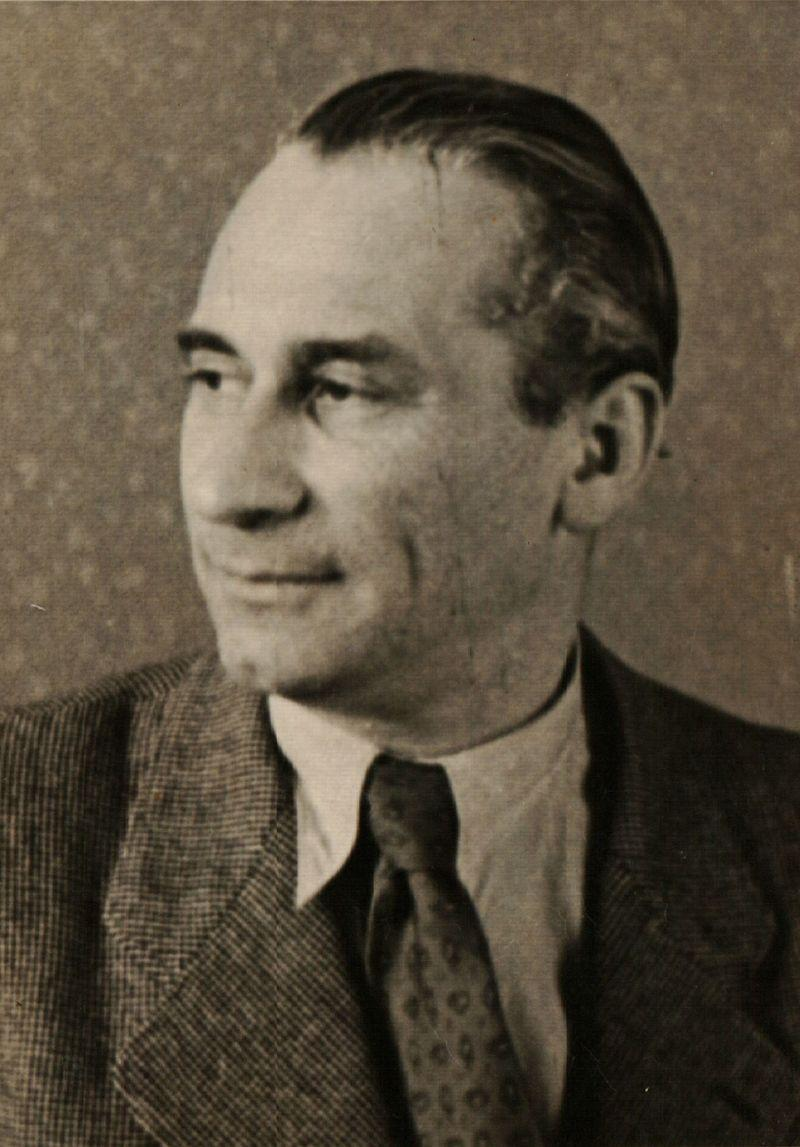
\includegraphics[width=1.5744in,height=2.2591in]{Kurzbiographien-img002.jpg}}
\end{figure}
Er wurde 1942 (genaues Datum unbekannt) mit seiner schwangeren Frau Valerie Ančerl (der Sohn Jan wurde am 28. Febr. 1943
im Ghetto geboren) in das Ghetto Theresienstadt deportiert. Dort nahm er aktiv am dortigen, von der SS geduldeten und
schließlich zu Propagandazwecken missbrauchten Kulturleben teil. 1943 gründete er ein \textit{Streichorchester}, mit
dem er wiederholt zwei Programme mit Werken von Georg Friedrich Händel, Johann Sebastian Bach, Wolfgang Amadé Mozart,
Josef Suk, Antonín Dvořák und Pavel Haas aufführte. Daneben wirkte er in den \textit{Kammervereinigungen} mit. Für ein
Konzert am 30. Apr. 1944 erstellte Ančerl eigens für sein Orchester ein Arrangement des vierten Satzes der 9. Symphonie
von Ludwig van Beethoven. Im selben Konzert dirigierte er die Theresienstädter Premiere von Dvořáks Streicherserenade
E-Dur. Zur Uraufführung dieser Komposition kam es ungeplant im Rahmen der Filmaufnahmen des Propagandafilms. Ančerl und
sein Orchester werden in einer Filmszene (Sequenz 34, 19:54min) gezeigt. Über die eigentliche Uraufführung am 13. Sept.
1944 berichtete Viktor Ullmann in einer Rezension, in der er dem jungen Ančerl hohe künstlerische Qualität
bescheinigte. Im September/Oktober 1944 wurden er mit seiner Familie in das KZ Auschwitz deportiert. Als Einziger
Überlebender seiner Familie wurde er im April 1945 im Arbeitslager Friedland, einem Außenlager des Konzentrationslagers
Groß-Rosen, von der roten Armee befreit.

Nach dem Krieg wurde er am 1.09.1947 zum Chefdirigent des Prager Rundfunksinfonieorchesters und im Oktober 1950 zum
künstlerischen Direktor der Tschechischen Philharmonie. In Folge der Niederschlagung des Prager Frühlings emigrierte er
im August 1968 nach Kanada und leitete dort bis 1972 das Toronto Symphony Orchestra.


\bigskip

\textbf{Sekundärliteratur:}

\begin{itemize}
\item Jaroslav Bužga: Ančerl, Karel. In: Ludwig Finscher (Hrsg.): Die Musik in Geschichte und Gegenwart. Zweite Ausgabe,
Personenteil, Band 1 (Aagard – Baez). Bärenreiter/Metzler, Kassel u. a. 1999, ISBN 3-7618-1111-X, Sp. 627–628
(Online-Ausgabe, für Vollzugriff Abonnement erforderlich)
\end{itemize}

\bigskip

\textbf{Internetquellen:}

\begin{itemize}
\item \url{http://www.ghetto-theresienstadt.de/pages/a/ancerlk.htm}
\item \url{https://www.lexm.uni-hamburg.de/object/lexm_lexmperson_00003301}
\item \url{https://collections.jewishmuseum.cz/index.php/Search/Index?search=Karel+ancerl} 
\item \url{https://de.wikipedia.org/wiki/Karel_An%C4%8Derl}
\end{itemize}

\bigskip

\textbf{Bildquelle:}

\begin{itemize}
\item \url{https://de.wikipedia.org/wiki/Karel_An%C4%8Derl#/media/Datei:BASA-1772K-1-2376-1-Karel_An%C4%8Derl.jpg}
\end{itemize}
\textbf{Dr. Leo Arje Lipmann Baeck} [geb. 23.05.1873 in Lissa (Provinz Posen); gest. 02.11.1956 in London (Vereinigtes
Königreich)] war ein deutscher Rabbiner und Präsident der Reichsvertretung der Deutschen Juden, sowie nach dem Krieg
Professor am Hebrew Union College in Cincinnati (USA).

\begin{figure}[h]
\centering
\lfbox[margin-top=0.1181in,margin-right=0.1181in,margin-bottom=0.1181in,margin-left=0.1181in,border-style=none,padding=0mm,vertical-align=top,raise=-0.9055in]{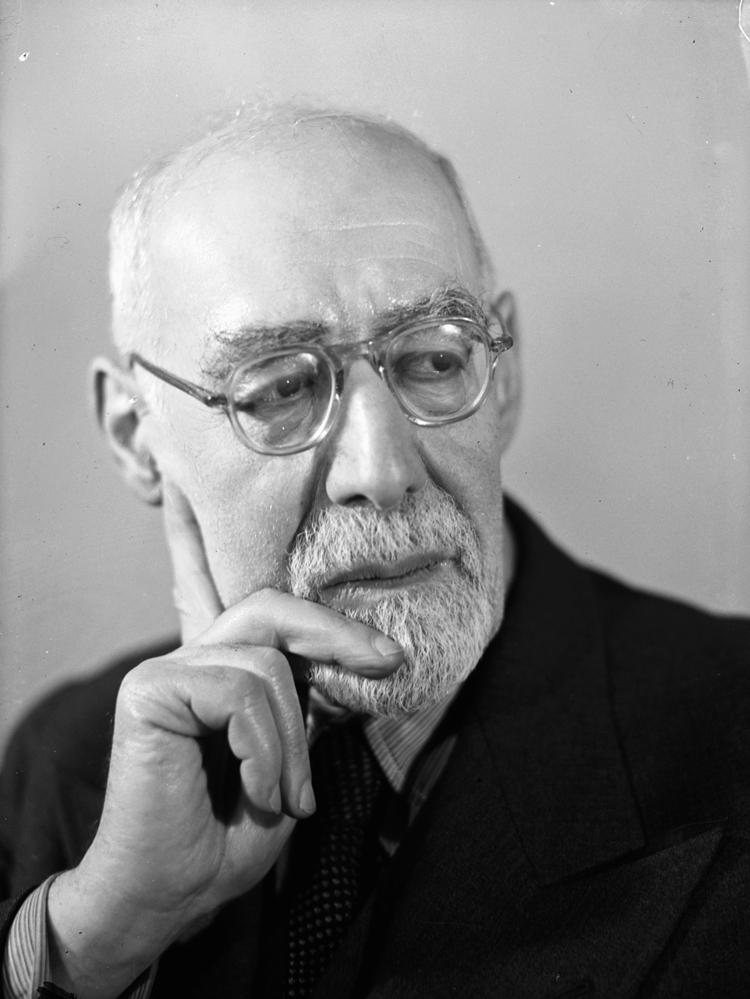
\includegraphics[width=1.5744in,height=2.098in]{Kurzbiographien-img003.jpg}}
\end{figure}
1895 wurde er Rabbiner in Oppeln an. In dieser Zeit entstand sein Hauptwerk \textit{Das Wesen des Judentums}, das 1905
erschien.Im Ersten Weltkriege Feldrabbiner. 1933 wurde er zum Präsident der \textit{Reichsvertretung der Deutschen
Juden} ernannt. Zugleich bis zur Schließung am 19.07.1942 war er Dozent an der Hochschule für die Wissenschaft des
Judentums. Mit seiner Frau Nathalie (geb. Hamburger) und seinen Kindern wurde er am 26.01.1943 mit dem Transport
10764/1–87 in das Ghetto Theresienstadt deportiert. Im Ghetto war er Mitglied im Ältestenrat. Außerdem initiierte er
zusammen mit Professor Maximilian Adler aus Prag und Professor Emil Utitz aus Halle eine \textit{Vortragsreihe}, die er
selbst mit einem Vortrag über Platon begann. Es existiert eine Liste seiner Vortragsthemen: Platon, Maimonides,
Spinoza, Kant, Mendelssohn, Hermann Cohen, Die jüdische Religionsphilosophie des Mittelalters, Die jüdische Mystik des
Mittelalters, Das Problem von Leib und Seele, Die Lebenseinheit in Leib und Seele, Der Sinn der Geschichte, Die
Geschichtsschreibung, Die Jahrhunderte von der Zerstörung des ersten bis zu der des zweiten Tempels, Die Zeit der
Makkabäer. Soweit bekannt, hielt er seinen letzten Vortrag mit dem Titel Galileo Galilei und das Ende des Mittelalters
am 23. Dezember 1944. Im Propagandafilm ist er zu sehen in der Sequenz \textit{Vortrag} (33). Er wurde am späten Abend
des 08.05.1945 in Theresienstadt durch die Rote Armee befreit. Nach dem Krieg emigrierte er am 05.06.1945 nach London.
Dort wirkte er als Präsident der \textit{Weltunion für progressives Judentum}. 1947 gründete er das später nach ihm
benannte\textit{ Institut zur Erforschung des Judentums in Deutschland seit der Aufklärung}.


\bigskip

\textbf{Eigene Werke:}

\begin{itemize}
\item Baeck, Leon: Werke: Hrsg. von Albert H. Friedlander, Bertold Klappert und Werner Licharz. Im Auftr. des Leo Baeck
Instituts, Gütersloher Verlagshaus, New York, Gütersloh 1998–2003 [Sonderausgabe: Gütersloher Verlagshaus, Gütersloh
2006].
\item Baeck, Leon: Das Wesen des Judentums. Nathansen \& Lamm, Berlin 1905. (Schriften der Gesellschaft zur Förderung
der Wissenschaft des Judentums).  
\item Baeck, Leon: Die jüdische religiöse Erziehung. In: Handbuch der Pädagogik. Hrsg. von Hermann Nohl. Band 3.
Langensalza [u. a.], 1930.  
\item Baeck, Leon: Romantische Religion. 1922.  
\item Baeck, Leon: Die Pharisäer. Schocken, Berlin 1934. (Bücherei des Schocken Verlags. 6.)  
\item Baeck, Leon: Religion und Weltfriede: Überwindung der Kriege. Sammelschrift mit Beiträgen von Leo Baeck, Günther
Dehn, Alfred Klee. Hrsg. von der Arbeitsgemeinschaft der Konfessionen für den Frieden. 1930. 
\item Baeck, Leon: Chaim Nachman Bialik. Eine Einführung in sein Leben und sein Werk. 1935.  
\item Baeck, Leon: Das Evangelium als Urkunde der jüdischen Glaubensgeschichte. 1938.  
\item Baeck, Leon: Der Sinn der Geschichte. 1946.  
\item Baeck, Leon: Maimonides, der Mann, sein Werk und seine Wirkung. 1954.  
\item Baeck, Leon: Dieses Volk – jüdische Existenz. 1955.  
\item Baeck, Leon: Aus drei Jahrtausenden. Wissenschaftliche Untersuchungen und Abhandlungen zur Geschichte des
jüdischen Glaubens. 1958.  
\item Baeck, Leon: Von Moses Mendelssohn zu Franz Rosenzweig: Typen jüdischen Selbstverständnisses in den letzten beiden
Jahrhunderten. 1958.  
\item Baeck, Leon: Paulus, die Pharisäer und das Neue Testament. Drei Aufsätze. Ner-Tamid Verlag, Frankfurt 1961.  
\item Baeck, Leon: Vorträge und Ansprachen. Mit einem Geleitwort von Leo Baeck. Herausgegeben von der Grossloge
Deutschland VIII U. O. B. B. 2., verb. Auflage, Maximilian Stein, Leo Baeck.  Zum 50jährigen Bestehen des Ordens Bne
Briss in Deutschland. U.O.B.B. (Enthält außerdem: Alfred Goldschmidt : Der deutsche Distrikt des Ordens Bne Briss.
Arthur Löwenstamm: Soziologie der Loge. Bruderworte. Zusammengestellt von Paul Rosenfeld.) Leo Baeck, Einleitung.  
\item Baeck, Leon: Geschichte der Juden. 3 Bände, 1954–1959, 1965.
\end{itemize}

\bigskip

\textbf{Sekundärliteratur:}

\begin{itemize}
\item Friedrich Wilhelm Bautz: Leo Baeck. In: Biographisch-Bibliographisches Kirchenlexikon (BBKL). Band 1, Bautz, Hamm
1975. 2., unveränderte Auflage Hamm 1990, ISBN 3-88309-013-1, Sp. 334–335.
\item Bastian Fleermann: „…das beste Rabbinat in Deutschland.“ Biografische Skizzen zu den Düsseldorfer Rabbinern von
1706 bis 1941. In: Düsseldorfer Jahrbuch, 81, 2011, S. 107–170.  
\item Albert H. Friedlander: Leo Baeck: Teacher of Theresienstadt. Overlook Press 1991, ISBN 978-0-87951-393-1 (Reprint
der Ausgabe 1973, 1. Aufl. 1968)  
\item Albert H. Friedlander: Leo Baeck, Leben und Lehre. Stuttgart 1973  
\item Elias H. Füllenbach: Rabbiner Leo Baeck – „Für die anderen zu leben und doch im Eigenen zu stehen“. In:
Düsseldorfer Persönlichkeiten. Hg. Edmund Spohr, Hatto Küffner, Kleve 2004 (= Düsseldorf. Eine Stadt zwischen Tradition
und Vision), S. 168–181.  
\item Eckhard Hansen, Florian Tennstedt (Hrsg.) u. a.: Biographisches Lexikon zur Geschichte der deutschen Sozialpolitik
1871 bis 1945. Band 2: Sozialpolitiker in der Weimarer Republik und im Nationalsozialismus 1919 bis 1945. Kassel
University Press, Kassel 2018, ISBN 978-3-7376-0474-1, S. 7 f. (Online, PDF; 3,9 MB).  
\item Maurice-Ruben Hayoun: Leo Baeck. Repräsentant des liberalen Judentums. WBG, Darmstadt 2015, ISBN
978-3-534-25758-4.  
\item Georg Heuberger, Fritz Backhaus, Leo Baeck 1873–1956. Aus dem Stamme von Rabbinern, Jüdischer Verlag im Suhrkamp,
Frankfurt am Main 2001, ISBN 3-633-54169-1.  
\item Walter Homolka: Jüdische Identität in der Modernen Welt. Leo Baeck und der deutsche Protestantismus. Kaiser,
Gütersloh 1994, ISBN 3-579-00259-7.  
\item Walter Homolka: Jüdisches Denken – Leo Baeck, Perspektiven für heute. Herder spektrum, Freiburg 2006, ISBN
978-3-451-05728-1.  
\item Walter Homolka, Elias H. Füllenbach: Leo Baeck – Eine Skizze seines Lebens. Gütersloher Verlagshaus, Gütersloh
2006, ISBN 978-3-579-06429-1.  
\item Walter Homolka, Elias H. Füllenbach: Rabbiner Leo Baeck. Ein Lebensbild. Zum Gedenken an Rabbiner Stanley Dreyfus.
Herausgegeben vom Centrum Judaicum. Verlag Hentrich \& Hentrich, Teetz 2009, ISBN 978-3-938485-84-2 (= Jüdische
Miniaturen Band 75).  
\item Ralf Koerrenz: Das Judentum als Lerngemeinschaft. Zur Konzeption einer pädagogischen Religion bei Leo Baeck.
Deutscher Studien-Verlag, Weinheim 1992 ISBN 3-89271-342-1.  
\item Reichshandbuch der deutschen Gesellschaft – Das Handbuch der Persönlichkeiten in Wort und Bild. Erster Band,
Deutscher Wirtschaftsverlag, Berlin 1930, ISBN 3-598-30664-4.  
\item Gerd Stecklina: »Was wir am Mitmenschen tun, ist Gottesdienst«. Leo Baeck 1873 – 1956, in Sabine Hering Hg., mit
Sandra Schönauer: Jüdische Wohlfahrt im Spiegel von Biographien. Schriftenreihe Geschichte der jüdischen Wohlfahrt in
Deutschland, 2. Hgg. Hering, Gudrun Maierhof, Ulrich Stascheit. Fachhochschulverlag, Frankfurt 2007 ISBN 3936065802 S.
66–73 (mit 1 Foto)
\end{itemize}

\bigskip


\bigskip

\textbf{Internetquellen:}

\begin{itemize}
\item \url{http://www.ghetto-theresienstadt.de/pages/b/baeckl.htm}
\item \url{https://www.leo-baeck-foundation.org/} 
\item \url{https://de.wikipedia.org/wiki/Leo_Baeck} 
\end{itemize}

\bigskip

\textbf{Bildquelle:}

\begin{itemize}
\item \url{https://www.leo-baeck-foundation.org/}
\end{itemize}
\textbf{Cornelia Cohen (geb. Spitzer)} [geb. unbekannt ; gest. unbekannt] war die Ehefrau von Cohen, David. Sie wurde
mit ihrem Ehemann David Cohen am 23.09.1943 in das Ghetto Theresienstadt deportiert. Ihre Rolle im Ghetto ist
unbekannt. Im Propoganadafilm ist sie in der Sequenz \textit{In der Bücherei} (32) und \textit{Abendessen} (37) zu
sehen. Sie wurde (vermutlich) zusammen mit ihrem Mann am späten Abend des 08.05.1945 in Theresienstadt durch die Rote
Armee befreit. 


\bigskip

\textbf{Prof. Dr. David Cohen} [geb. 31.12.1882 in Deventer (Niederlande); gest. 03.09.1967 in Amsterdam (Niederlande)]
war ein niederländischer Althistoriker, Papyrologe und Vorsitzender des Judenrats der Niederlande zur Zeit des
Nationalsozialismus.

\begin{figure}[h]
\centering
\lfbox[margin-top=0.1181in,margin-right=0.1181in,margin-bottom=0.1181in,margin-left=0.1181in,border-style=none,padding=0mm,vertical-align=top,raise=-0.9055in]{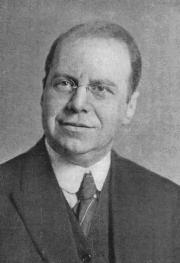
\includegraphics[width=1.5744in,height=2.2984in]{Kurzbiographien-img004.jpg}}
\end{figure}
Von 1924 bis 1926 war er Professor für Altertumswissenschaften in Leiden und von 1926 bis zu seiner Emeritierung 1953
ordentlicher Professor für Alte Geschichte an der Universität von Amsterdam. Er galt als Fachmann für Papyrologie. Nach
der Besetzung der Niederlande durch das Deutsche Reich gehörte er zu den Mitbegründern eines jüdischen
Koordinierungsausschusses. 

Er wurde mit seiner Frau Cornelia Spitzer am 23.09.1943 als einer der letzten in den Niederlanden verbliebenen Juden
über das Durchgangslager Westerbork in das Ghetto Theresienstadt deportiert. Im Ghetto war er Mitglied im Ältestenrat.
Im Propoganadafilm ist sie in der Sequenz \textit{In der Bücherei} (32) und \textit{Abendessen} (37) zu sehen. Er wurde
am späten Abend des 08.05.1945 in Theresienstadt durch die Rote Armee befreit. Zurück in den Niederlanden nahm er nach
erfolglosen Ermittlungsverfahren wegen Kollaboration 1950 seine Position als Professor der Alten Geschichte an der
Universität von Amsterdam wieder auf.


\bigskip

\textbf{Sekundärliteratur:}

\begin{itemize}
\item Hans G. Adler: Theresienstadt. Das Antlitz einer Zwangsgemeinschaft 1941–1945. Nachwort Jeremy Adler. Wallstein,
Göttingen 2005 ISBN 3-89244-694-6 (Reprint der 2. verb. Auflage Mohr-Siebeck, Tübingen 1960. 1. Aufl. ebd. 1955)
\item Israel Gutman (Hrsg.): Enzyklopädie des Holocaust – Die Verfolgung und Ermordung der europäischen Juden. Piper
Verlag, München/Zürich 1998, 3 Bände, ISBN 3-492-22700-7  
\item Anna Hájková: Die Juden aus den Niederlanden in Theresienstadt. In: Theresienstädter Studien und Dokumente 2002,
S. 135–201.  
\item Pieter Herman Schrijvers: Rome, Athene, Jeruzalem. Leven en werk van prof. dr. David Cohen. Historische
uitgeverij, Groningen 2000. – Rez. von: J. C. H. Blom, in: BMGN – Low Countries Historical Review 116, 2001, afl. 2, S.
198–203, (online) (PDF).
\end{itemize}

\bigskip

\textbf{Internetquellen:}

\begin{itemize}
\item \url{http://www.ghetto-theresienstadt.de/pages/c/cohend.htm} 
\item \url{http://resources.huygens.knaw.nl/bwn1880-2000/lemmata/bwn3/cohend} (JW Schulte Nordholt: 'Cohen, David
(1882-1967)', in: Huygens: Biografischen Wörterbuch der Niederlande)
\item \url{https://de.wikipedia.org/wiki/David_Cohen_(Historiker}) 
\end{itemize}

\bigskip

\textbf{Bildquelle:}

\begin{itemize}
\item \url{http://resources.huygens.knaw.nl/bwn1880-2000/lemmata/bwn3/cohend}
\end{itemize}
\textbf{Elisabeth Czech} [geb. unbekannt in der Tschecheslowakei (vermutlich); gest. nach 1948 in London (Vereinigtes
Königreich, vermutlich)] war die Ehefrau von Dr. Ludwig Czech, dem ehemaligen. Minister für Wohlfahrt und Gesundheit in
Prag.

Sie wurde am 22.03.1942 in das Ghetto Theresienstadt deportiert. Ihre Rolle im Ghetto ist unbekannt. Im Propoganadafilm
ist sie in der Sequenz \textit{Konzert} (34) zu sehen. Sie wurde am späten Abend des 8.05.1945 in Theresienstadt durch
die Rote Armee befreit. Über ihr weiteres Leben ist soweit nichts bekannt.


\bigskip


\bigskip

\textbf{Internetquellen:}

\begin{itemize}
\item \url{https://wiener.soutron.net/Portal/Default/en-GB/recordview/index/106300}
\end{itemize}

\bigskip


\bigskip

\textbf{Dr. Heinrich Dessauer }[geb. 08.09.1883 in Wien (Österreich-Ungarn); gest. nach 12.10.1944 im KZ Auschwitz
(Generalgouvernement Polen)] war ein österreichischer Rechtsanwalt, Gerichtsdolmetscher und Mitglied des Ältestenrates
der Juden in Wien. Seit 1939 bis zu seiner Deportation war er Leiter des Rechtsbüros der Jüdischen Kultusgemeinde in
Wien

\begin{figure}[h]
\centering
\lfbox[margin-top=0.1181in,margin-right=0.1181in,margin-bottom=0.1181in,margin-left=0.1181in,border-style=none,padding=0mm,vertical-align=top,raise=-0.9055in]{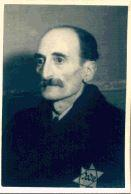
\includegraphics[width=1.5744in,height=2.3264in]{Kurzbiographien-img005.jpg}}
\end{figure}
Er wurde mit seiner Frau Marietta Dessauer (geb. Friedmann) und seinen 2 Kindern am 29.01.1943 in das Ghetto
Theresienstadt deportiert. Seine Rolle im Ghetto ist unbekannt. Im Propoganadafilm ist er zu sehen in der Sequenz
Konzert (34). Am 14.10.1944 wurde er in das KZ Auschwitz deportiert und dort ermordet.


\bigskip

\textbf{Internetquellen:}

\begin{itemize}
\item \url{http://www.ghetto-theresienstadt.de/pages/d/dessauerh.htm} 
\end{itemize}

\bigskip

\textbf{Bildquelle:}

\begin{itemize}
\item \url{http://www.ghetto-theresienstadt.de/images/prominente/Bild109.gif}
\end{itemize}
\textbf{Dr. Paul Maximilian Eppstein} [geb. 04.03.1902 in Ludwigshafen (Deutsches Reich); gest. 27./28.11.1944 im Ghetto
Theresienstadt (Tschechoslowakei)] war ein deutscher Soziologe. 

\begin{figure}[h]
\centering
\lfbox[margin-top=0.1181in,margin-right=0.1181in,margin-bottom=0.1181in,margin-left=0.1181in,border-style=none,padding=0mm,vertical-align=top,raise=-0.9055in]{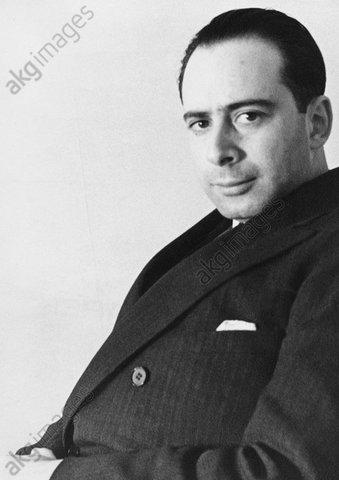
\includegraphics[width=1.5744in,height=2.2311in]{Kurzbiographien-img006.jpg}}
\end{figure}
1928 wurde er Leiter der Volkshochschule Mannheim und lehrte in den 1930er Jahren an der Hochschule für die Wissenschaft
des Judentums in Berlin Soziologie. Ab 1933 war er Vertreter der Reichsvereinigung der Juden in Deutschland. Er wurde
mit seiner Frau, der Psychologin und Sozialarbeiterin Hedwig Eppstein (geb. Strauß) und zusammen mit Leo Baeck am
26.01.1943 mit dem Transport I/86 in das Ghetto Theresienstadt deportiert. Dort wurde er als Nachfolger von Jakob
Edelstein zum \textit{Judenältesten} ernannt. In dieser Funktion solcher war er unter anderem gezwungen, Deportationen
in die Vernichtungslager mit vorzubereiten. Im Propoganadafilm ist er in der Fußballszene (10), die bereits am 1.09.44
gedreht worden war, zu sehen. Am 27. oder 28.09.1944 wurde er in der Kleinen Festung Theresienstadt erschossen. Seine
Frau Hedwig wurde am 28.10.1944 nach Auschwitz deportiert und dort ermordet. 


\bigskip

\textbf{Eigene Werke:}

\begin{itemize}
\item \textit{Die Symptomatik in der Konjunkturforschung 1933}
\end{itemize}

\bigskip

\textbf{Sekundärliteratur:}

\begin{itemize}
\item John F. Oppenheimer (Red.) u. a.: Lexikon des Judentums. 2. Auflage. Bertelsmann Lexikon Verlag, Gütersloh u. a.
1971, ISBN 3-570-05964-2, Sp. 187.  
\item Karl Otto Watzinger: Geschichte der Juden in Mannheim 1650–1945. Kohlhammer, Stuttgart 1984, ISBN 3-17-008696-0,
S. 89–92.  
\item Israel Gutman (Hrsg.): Enzyklopädie des Holocaust – Die Verfolgung und Ermordung der europäischen Juden. 3 Bände,
Piper Verlag, München/Zürich 1998, ISBN 3-492-22700-7.  
\item Beate Meyer: Tödliche Gratwanderung – Die Reichsvereinigung der Juden in Deutschland zwischen Hoffnung, Zwang,
Selbstbehauptung und Verstrickung (1939–1945). Göttingen 2011, ISBN 978-3-8353-0933-3.  
\item Wolfgang Benz: Deutsche Juden im 20. Jahrhundert : eine Geschichte in Porträts. München : Beck, 2011, ISBN
978-3-406-62292-2, darin: „Judenältester“ in Theresienstadt: Paul Eppstein, S. 65–77  
\item Claus-Dieter Krohn: Eppstein, Paul. In: Harald Hagemann, Claus-Dieter Krohn (Hrsg.): Biographisches Handbuch der
deutschsprachigen wirtschaftswissenschaftlichen Emigration nach 1933. Band 1: Adler–Lehmann. Saur, München 1999, ISBN
3-598-11284-X, S. 142–143.  
\item Eppstein, Paul, in: Joseph Walk (Hrsg.): Kurzbiographien zur Geschichte der Juden 1918–1945. München : Saur, 1988,
ISBN 3-598-10477-4, S. 81f.  
\item Eppstein, Hedwig, in: Joseph Walk (Hrsg.): Kurzbiographien zur Geschichte der Juden 1918–1945. München : Saur,
1988, ISBN 3-598-10477-4, S. 81
\end{itemize}

\bigskip


\bigskip

\textbf{Internetquellen:}

\begin{itemize}
\item \url{http://www.ghetto-theresienstadt.de/pages/e/eppsteinp.htm}  
\item \url{https://www.holocaust.cz/de/opferdatenbank/opfer/9797-hedwig-eppstein/} 
\item \url{https://de.wikipedia.org/wiki/Paul_Eppstein} 
\end{itemize}

\bigskip

\textbf{Bildquelle:}

\begin{itemize}
\item \url{https://www.geni.com/photo/view/6000000050897081907?album_type=photos_of_me&photo_id=6000000050955430138} 
\end{itemize}
\textbf{Karel Fischer }[geb. 01.06.1913 in Zdíkov (Tschecheslowakei); gest. 28.09.1944 im KZ Auschwitz
(Generalgouvernement Polen)] war ein tschechoslowakischer Dirigent.

\begin{figure}[h]
\centering
\lfbox[margin-top=0.1181in,margin-right=0.1181in,margin-bottom=0.1181in,margin-left=0.1181in,border-style=none,padding=0mm,vertical-align=top,raise=-0.9055in]{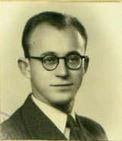
\includegraphics[width=1.5744in,height=1.8181in]{Kurzbiographien-img007.jpg}}
\end{figure}
Er wurde am 13.07.42 mit dem Transport Aaq in das Ghetto Theresienstadt deportiert. Seine Rolle im Ghetto ist unbekannt.
Er wirkte an der musikalischen Umsetzung des Propagandafilms (Felix Mendelssohn-Bartholdy: Elias \& Sommernachtstraum
\& Violinsonate) mit und ist in der Sequenz Konzert (1) zu sehen. Am 28.09.1944 wurde er in das KZ Auschwitz deportiert
und dort ermordet.


\bigskip

\textbf{Internetquellen:}

\begin{itemize}
\item \url{http://www.musiques-regenerees.fr/Terezin/AutresCompositeurs/GerronFilm.html}  
\item \url{https://yvng.yadvashem.org/nameDetails.html?language=en&itemId=4760579&ind=1}  
\item
\url{https://www.holocaust.cz/de/datenbank-der-digitalisiertendokumenten/dokument/120792-fischer-karel-pripusteni-k-ridicske-zkousce/}

\end{itemize}

\bigskip


\bigskip

\textbf{Bildquelle:}

\begin{itemize}
\item
\url{https://www.holocaust.cz/de/datenbank-der-digitalisierten-dokumenten/dokument/120792-fischer-karel-pripusteni-k-ridicske-zkousce/}

\end{itemize}
\textbf{Dr. Max Moses Friediger} [geb. 09.04.1884 in Budapest (Ungarn); gest. 09.04.1947 in Kopenhagen (Dänemark)] war
ein dänischer Rabbiner. 

\begin{figure}[h]
\centering
\lfbox[margin-top=0.1181in,margin-right=0.1181in,margin-bottom=0.1181in,margin-left=0.1181in,border-style=none,padding=0mm,vertical-align=top,raise=-0.9055in]{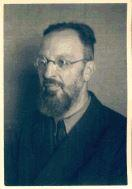
\includegraphics[width=1.5744in,height=2.2555in]{Kurzbiographien-img008.jpg}}
\end{figure}
Er war Rabbiner in Pohrlitz (1911-1913) und Oderberg (1913-1919). Im Ersten Weltkrieg war er Feldrabbiner der k. u. k.
Armee (1916-1918). Von 1920 bis 1947 war er in Kopenhagen königlich-dänischer Oberrabbiner. 

Er wurde mit seiner Frau Fanny Friediger (geb. Seegall) und seinen 2 Kindern wurde er am 29.08.1943 verhaftet, im Lager
Horserød interniert und am 06.10.43 mit dem Transport in das Ghetto Theresienstadt deportiert. Im Ghetto war er
Mitglied im Ältestenrat, sowie Mitarbeiter der Fürsorge.Im Propoganadafilm ist er in der Sequenz \textit{Terrasse} (4)
zu sehen. Mitte April 1945 wurde er im Rahmen der Rettungsaktion der \textit{Weißen Busse} durch das Schwedische Rote
Kreuz mit weiteren dänischen Häftlingen aus Theresienstadt nach Schweden evakuiert. Nach dem Krieg war er erneut bis zu
seinem Tod königlich-dänischer Oberrabbiner.


\bigskip

\textbf{Eigene Werke:}

\begin{itemize}
\item Max Friediger: Theresienstadt, Kopenhagen 1946 (dänisch)
\end{itemize}

\bigskip

\textbf{Sekundärliteratur:}

\begin{itemize}
\item Hans Günther Adler: Theresienstadt. Das Antlitz einer Zwangsgemeinschaft 1941-1945 Nachwort Jeremy Adler.
Wallstein, Göttingen 2005 ISBN 3-89244-694-6 (Reprint der 2. verb. Auflage Mohr-Siebeck, Tübingen 1960. 1. Aufl. ebd.
1955)  
\item Axel Feuß: Das Theresienstadt-Konvolut, Altonaer Museum in Hamburg, Dölling und Galitz Verlag, Hamburg/München
2002, ISBN 3-935549-22-9. 
\item Esriel Hildesheimer, Mordechai Eliav: Das Berliner Rabbinerseminar 1873-1938, Berlin 2008, ISBN 9783938485460, S.
115
\item Leo Goldberger: \textit{The Rescue Of The Danish Jews: Moral Courage Under Stress.} New York New York University
Press, 1988. S. 71 
\end{itemize}

\bigskip


\bigskip

\textbf{Internetquellen:}

\begin{itemize}
\item \url{http://www.ghetto-theresienstadt.de/pages/f/friedigerm.htm} 
\item \url{https://de.wikipedia.org/wiki/Max_Friediger} 
\end{itemize}

\bigskip

\textbf{Bildquelle:}

\begin{itemize}
\item \url{http://www.ghetto-theresienstadt.de/images/prominente/Bild101.gif} 
\end{itemize}
\textbf{Dr. Desider Friedmann} () [geb. 24.11.1880 in Boskovice (Österreich-Ungarn); gest. 1944 (Oktober) im KZ
Auschwitz (Generalgouvernement Polen)] war ein österreichischer Rechtsanwalt und Präsident der Israelitischen
Kultusgemeinde Wien (1933-1938).

\begin{figure}[h]
\centering
\lfbox[margin-top=0.1181in,margin-right=0.1181in,margin-bottom=0.1181in,margin-left=0.1181in,border-style=none,padding=0mm,vertical-align=top,raise=-0.9055in]{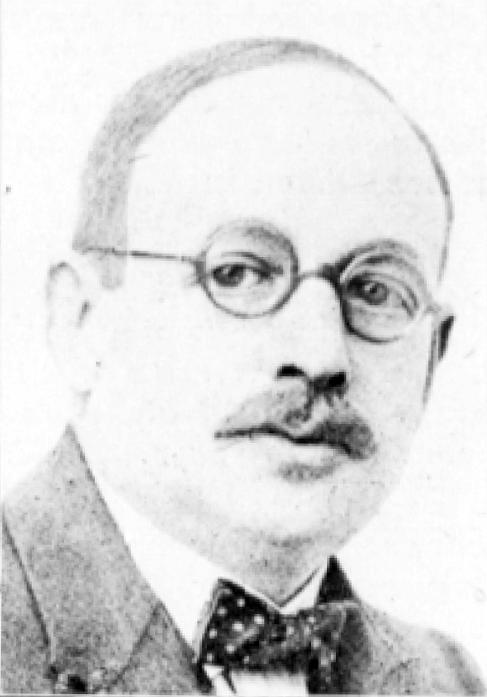
\includegraphics[width=1.5744in,height=2.2516in]{Kurzbiographien-img009.jpg}}
\end{figure}
Nach dem Anschluss Österreichs am 18.03.1938 verhaftet, Anfang April 1938 in das KZ Dachau eingeliefert, vom 25.09.1938
bis 10.05.1939 im KZ Buchenwald inhaftiert, wurde er mit seiner Frau Ella (geb. Stiassni) am 24.11.1942 in das Ghetto
Theresienstadt deportiert. Im Ghetto war er Mitglied im Ältestenrat, Stellvertreter des Judenältesten Jakob Eppstein
sowie Leiter der \textit{Bank der Jüdischen Selbstverwaltung}. Die Nazis wollten mit der Bank den Schein der Seriosität
wahren. So musste er während des Besuchs der Kommission des Internationalen Roten Kreuzes den biederen Bankmenschen
spielen. Er hielt vor der Kommission einen Vortrag, bot Zigarren an und wurde von Haindl als Chauffeur in einem
Mercedes Kompressor durchs Ghetto gefahren. Auch im Propagandafilm musste er den Bankdirektor spielen (22) und ist auch
in der Sequenz \textit{Bücherei} (32) zu sehen. Gemeinsam mit seiner Ehefrau wurde er im Oktober 1944 mit einem der
letzten Transporte nach Auschwitz deportiert und dort ermordet. Mit einem der letzten Transporte wurde er gemeinsam mit
seiner Frau im Oktober 1944 nach Auschwitz deportiert und dort ermordet


\bigskip

\textbf{Sekundärliteratur:}

\begin{itemize}
\item Avraham Barkai, Paul Mendes-Flohr, Steven M Lowenstein: Deutsch-jüdische Geschichte in der Neuzeit. C. H. Beck,
1997, ISBN 3-406-39706-9. 
\item Hans Günther Adler: Theresienstadt. Das Antlitz einer Zwangsgemeinschaft 1941–1945. Nachwort Jeremy Adler.
Wallstein, Göttingen 2005, ISBN 3-89244-694-6 (Reprint der 2., verb. Auflage. Mohr-Siebeck, Tübingen 1960. 1. Aufl.
ebenda 1955). 
\item Claims Resolution Tribunal: Aktenzeichen: CV96-4849 betreffend das Konto des Kontoinhabers Desider Friedmann.
(Inoffizielle Übersetzung des englischen Originaltextes) (pdf; 26 kB) 
\item Marianne Enigl: In jedem Fall trägt der Jude die Verantwortung (Teil 2). In: Profil. Ausgabe 28, 9. Juli 2007, S.
36 ff.
\item Marianne Enigl: Zeitgeschichte: Die Bürokratie der Opfer - Österreichs Juden: Ihr Leben und ihr Sterben. (Teil 1).
In: Profil. Ausgabe 27, 2. Juli 2007, S. 30 ff.
\end{itemize}

\bigskip


\bigskip

\textbf{Internetquellen:}

\begin{itemize}
\item \url{http://www.ghetto-theresienstadt.de/pages/f/friedmannd.htm} 
\item  \url{http://www.yadvashem.org/yv/en/exhibitions/last_portrait/images/karlinsky/05.jpg} 
\item \url{https://de.wikipedia.org/wiki/Desider_Friedmann} 
\end{itemize}

\bigskip

\textbf{Bildquelle:}

\begin{itemize}
\item \url{https://de.wikipedia.org/wiki/Desider_Friedmann#/media/Datei:Desider_Friedmann.jpg} 
\end{itemize}
\textbf{Dr. Heinrich Gans} [geb. 15.10.1874 in Eureka (Kansas, USA); gest. nach Juni/Juli 1944], deutscher Staatsbürger,
war Wirklicher Hofrat der Wiener Polizeidirektion i.R..

\begin{figure}[h]
\centering
\lfbox[margin-top=0.1181in,margin-right=0.1181in,margin-bottom=0.1181in,margin-left=0.1181in,border-style=none,padding=0mm,vertical-align=top,raise=-0.9055in]{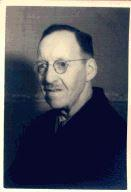
\includegraphics[width=1.5744in,height=2.3063in]{Kurzbiographien-img010.jpg}}
\end{figure}
Er arbeitete 35 Jahre bei der Wiener Polizeidirektion, davon 10 Jahre als selbständiger Referent der Kriminalpolizei im
Sicherheitsbüro. Zuletzt war er Leiter des Vereins- und Versammlungswesens.

Er wurde (vermutlich) mit seiner Frau Olga (geb. Otte) und seine Kinder am 25.09.1942 mit dem Transport IV/11  in das
Ghetto Theresienstadt deportiert. Seine Rolle im Ghetto ist unbekannt. Im Propoganadafilm ist er in der Sequenz Konzert
(34) zu sehen. Er muss nach 1944 ermordet worden sein.


\bigskip

\textbf{Internetquellen:}

\begin{itemize}
\item \url{http://www.ghetto-theresienstadt.de/pages/g/gansh.htm}
\item \url{https://www.holocaust.cz/de/opferdatenbank/opfer/61605-heinrich-gans/} 
\end{itemize}

\bigskip

\textbf{Bildquelle:}

\begin{itemize}
\item \url{http://www.ghetto-theresienstadt.de/images/prominente/Bild96.gif}
\end{itemize}
\textbf{Kurt Gerron} (eigtl. Gerson) [geb. 11.05.1897 in Berlin (Deutsches Reich); gest. 28.10.1944 im KZ Auschwitz
(Generalgouvernement Polen)] war ein deutscher Schauspieler, Sänger, Regisseur.

\begin{figure}[h]
\centering
\lfbox[margin-top=0.1181in,margin-right=0.1181in,margin-bottom=0.1181in,margin-left=0.1181in,border-style=none,padding=0mm,vertical-align=top,raise=-0.9055in]{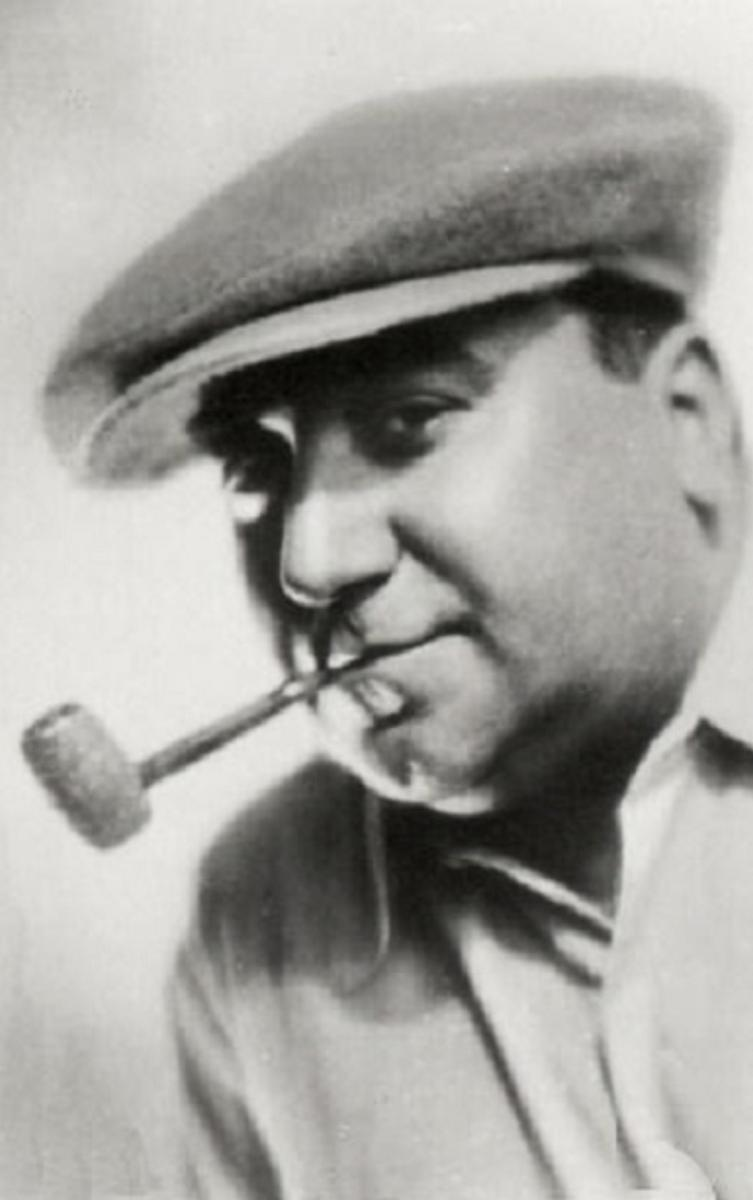
\includegraphics[width=1.5744in,height=2.5071in]{Kurzbiographien-img011.jpg}}
\end{figure}
Wandte sich in den 1920ern der Schauspielerei zu - Berliner Reinhardt-Bühnen (1920-1925) und Nebenrollen in Stummfilmen.
Führte ab 1926 selbst Regie. Sein wohl größte Erfolg war die Rolledes Zauberkünstlers Kiepert in Josef von Sternbergs
Der blaue Engel (1930). Bis 1933 wirkte er in 60 Filmen mit. Nach der Machtergreifung der Nationalsozialisten floh er
zunächst mit seiner Frau Olga (geb. Meyer) von Paris, von da über Österreich und Italien nach Amsterdam. Nach der
Besetzung der Niederlande wurden er und seine Frau über das Durchgangslager Westerbork am 25.02.44 mit dem Transport
XXIV/4 in das Ghetto Theresienstadt deportiert. Im Ghetto war er Gründer und Leiter des \textit{Ghetto-Kabaretts
Karussell}. Er wurde verpflichtet den den vorgeblich dokumentarischen Propagandafilm als Regisseur zu inszenieren. Nach
Abschluss der Filmarbeiten wurden er im Oktober 1944 nach Auschwitz transportiert und dort vergast.


\bigskip

\textbf{Eigene Werke (als Regisseur):}

\begin{itemize}
\item 1926: Der Liebe Lust und Leid  
\item 1931: Der Stumme von Portici  
\item 1931: UFA-Kabarett (Filmreihe mit insgesamt 6 Folgen)  
\item 1931: Meine Frau, die Hochstaplerin  
\item 1932: Es wird schon wieder besser  
\item 1932: Ein toller Einfall  
\item 1932: Der weiße Dämon  
\item 1933: Heut’ kommt’s drauf an  
\item 1933: Kind, ich freu’ mich auf Dein Kommen (beendet durch Erich von Neusser)  
\item 1933: Une femme au volant  
\item 1933: Incognito  
\item 1934: Bretter, die die Welt bedeuten  
\item 1935: Das Geheimnis der Mondscheinsonate (Het mysterie van de Mondscheinsonate)  
\item 1936: Merijntje Gijzen’s Jeugd  1936: Eeen dag bij de A.V.R.O.(Dokumentarfilm)  
\item 1937: De drie wensen  
\item 1944: Theresienstadt. Ein Dokumentarfilm aus dem jüdischen Siedlungsgebiet 
\end{itemize}

\bigskip

\textbf{Sekundärliteratur:}

\begin{itemize}
\item Barbara Felsmann, Karl Prümm: Kurt Gerron – Gefeiert und gejagt. 1897–1944. Das Schicksal eines deutschen
Unterhaltungskünstlers. Berlin, Amsterdam, Theresienstadt, Auschwitz (= Beiträge zu Theater, Film und Fernsehen aus dem
Institut für Theaterwissenschaft der Freien Universität Berlin. Bd. 7 = Reihe deutsche Vergangenheit. Nr. 63). Edition
Hentrich, Berlin 1992, ISBN 3-89468-027-X.  
\item Ulrich Liebe: Verehrt, Verfolgt, Vergessen. Schauspieler als Naziopfer. Beltz Quadriga, Weinheim u. a. 1992, ISBN
3-88679-197-1.  
\item Roy Kift: Camp Comedy. A play featuring original cabaret songs from Gerron’s Karussell cabaret, and dealing with
Gerron’s moral dilemma in making the propaganda film for Goebbels. In: Robert Skloot (Hrsg.): The theatre of the
Holocaust. Band 2: Six plays. University of Wisconsin Press, Madison WI u. a. 1999, ISBN 0-299-16274-5
\item Katja B. Zaich: „Ein Emigrant erschiene uns sehr unerwünscht.“ K. G. als Filmregisseur, Schauspieler und
Cabaretier in den Niederlanden. In: Claus-Dieter Krohn, Lutz Winckler, Irmtrud Wojak, Wulf Koepke (Hrsg.): Film und
Fotografie (= Exilforschung. Ein internationales Jahrbuch. Bd. 21). Edition Text und Kritik, München 2003, ISBN
3-88377-746-3, S. 112–128.  
\item Charles Lewinsky: Gerron. Roman. Nagel \& Kimche, Zürich 2011, ISBN 978-3-312-00478-2.  
\item Kay Weniger: „Es wird im Leben dir mehr genommen als gegeben ….“ Lexikon der aus Deutschland und Österreich
emigrierten Filmschaffenden 1933 bis 1945. Eine Gesamtübersicht. ACABUS-Verlag, Hamburg 2011, ISBN 978-3-86282-049-8,
S. 185–188.
\end{itemize}

\bigskip


\bigskip

\textbf{Internetquellen:}

\begin{itemize}
\item \url{http://www.ghetto-theresienstadt.de/pages/g/gerronk.htm} 
\item \url{https://de.wikipedia.org/wiki/Kurt_Gerron} 
\end{itemize}

\bigskip

\textbf{Bildquelle:}

\begin{itemize}
\item \url{https://www.holocaust.cz/de/datenbank-der-digitalisierten-dokumenten/dokument/444305-kurt-gerron/} 
\end{itemize}
\textbf{Dr. Rolf Grabower} [geb. 21.05.1883 in Berlin (Deutsches Reich); gest. 07.03.1963 in München (Bundesrepublik
Deutschland)] war ein deutscher Jurist. Als Richter am Reichsfinanzhof und Steuerrechtler wurde er zum 'Vater' der
Umsatzsteuer.

\begin{figure}[h]
\centering
\lfbox[margin-top=0.1181in,margin-right=0.1181in,margin-bottom=0.1181in,margin-left=0.1181in,border-style=none,padding=0mm,vertical-align=top,raise=-0.9055in]{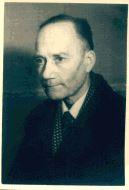
\includegraphics[width=1.5744in,height=2.322in]{Kurzbiographien-img012.jpg}}
\end{figure}
1934 wurde er als Oberster Richter zum (politisch einflusslosen) Reichsfinanzhof nach München versetzt. Vom 3.04.1941
bis Juli 1945 war er anch eigenem Bekunden Erdarbeiter, Hilfsarbeiter bei den Maurern, Leiter einer Fabrik,
Arbeitsrichter, Verwaltungsrichter, Leiter des jüdischen Arbeitseinsatzes im Lager Milpertshofen und in einer
Flachsröste in Lohhof. 

Er wurden am 19.06.1942 mit dem Transport 341–II/7 in das Ghetto Theresienstadt deportiert. Im Ghetto war er in der
\textit{Arbeitszentrale} beschäftigt, gehörte dem \textit{Bankbeirat} zu und pfelgte Kontakte zur
\textit{Manes-Gruppe}. Im Propoganadafilm ist er in der Sequenz \textit{Freilichtvarietee} (22) zu sehen. Er wurde am
späten Abend des 08.05.1945 in Theresienstadt durch die Rote Armee befreit. Er blieb freiwillig noch zwei Monate in
Theresienstadt, um bei der Abwicklung des Lagers zu helfen. Dannach war er wieder höchster Reichsrichter beim nun
Bayerischen Obersten Finanzgerichtshof in München. Am 18. Oktober 1945 wurde er zum Oberfinanzpräsidenten in Nürnberg
ernannt. Ende März 1952 wurde er pensioniert. 


\bigskip

\textbf{Eigene Werke:}

\begin{itemize}
\item mit Johannes Popitz: Die Geschichte der Umsatzsteuer und ihre gegenwärtige Gestaltung im Inland und im Ausland.
Carl Heymanns Verlag, Berlin 1925.  
\item Steuerverwaltung und Ethik  
\item Die ethische Betrachtungsweise im Steuerrecht  
\item Preußens Steuern vor und nach den Befreiungskriegen. Liebmann-Verlag, Berlin 1932.  
\item Die Buch- und Betriebsprüfung der Reichsfinanzverwaltung. Spaeth \& Linde, Berlin Wien 1932.  
\item Handbuch des Steuerstrafrechts und Steuerstrafverfahrensrechts. Stoytscheff, Nürnberg 1949.  
\item mit Theodor Eschenburg: Klugheitsregeln der Verwaltung. Ämterpatronage im Parteienstaat. Politische Studien
(Hanns-Seidel-Stiftung) 61 (1956)  
\item Bismarck und die Steuern. Zugleich ein Beitrag zur Lehre von der Tradition im Steuerwesen. FinanzArchiv 1962.
\end{itemize}

\bigskip

\textbf{Sekundärliteratur:}

\begin{itemize}
\item Martin Friedenberger, Klaus-Dieter Gössel, Eberhard Schönknecht (Hrsg.): Die Reichsfinanzverwaltung im
Nationalsozialismus. Darstellung und Dokumente. Temmen, Bremen 2002, ISBN 3-86108-377-9 (Veröffentlichungen der Gedenk-
und Bildungsstätte Haus der Wannsee-Konferenz 1).  
\item Werner Nigbur (Hrsg.): Wenn im Amte, arbeite, wenn entlassen, verbirg dich. Prof. Dr. iur. Dr. phil. Rolf Grabower
„Dreivierteljude“, Überlebender der Shoa, Theresienstadt. In Zeugnissen aus der Finanzgeschichtlichen Sammlung der
Bundesfinanzakademie. Ein Lesebuch und Materialband. Bundesfinanzakademie im Bundesministerium der Finanzen, Brühl
2010.  ofd aktuell. Nachrichten der Oberfinanzdirektion Nürnberg. Nr. 2/83.  
\item Alfons Pausch: Rolf Grabower – Architekt des Betriebsprüfungsdienstes im Interesse der Gleichmäßigkeit der
Besteuerung. Steuer und Studium 1992, ISSN 0173-1599, S. 43 ff.  Erich Stockhorst: 5000 Köpfe. Wer war was im 3. Reich.
Arndt, Kiel 2000, ISBN 3-88741-116-1 (Unveränderter Nachdruck der ersten Auflage von 1967).  
\item Christian Scheer: Grabower, Rudolf. In: Harald Hagemann, Claus-Dieter Krohn (Hrsg.): Biographisches Handbuch der
deutschsprachigen wirtschaftswissenschaftlichen Emigration nach 1933. Band 1: Adler–Lehmann. Saur, München 1999, ISBN
3-598-11284-X, S. 195–197.  
\item Johanna Rakebrand: „Grabower {\textbar} Popitz. Zwei uneindeutige Deutsche“, Myops 30 (2017), München, C.H. Beck,
S. 61–71.
\end{itemize}

\bigskip


\bigskip

\textbf{Internetquellen:}

\begin{itemize}
\item \url{http://www.ghetto-theresienstadt.de/pages/g/grabowerr.htm} 
\item \url{https://de.wikipedia.org/wiki/Rolf_Grabower} 
\end{itemize}

\bigskip

\textbf{Bildquelle:}

\begin{itemize}
\item \url{http://www.ghetto-theresienstadt.de/images/prominente/Bild91.gif} 
\end{itemize}
\textbf{Dr. Georg Gradnauer} [geb. 16.11.1866 in Magdeburg (Deutsches Reich); gest. 18.11.1946 in Berlin-Schlachtensee
(Sowjetische Besatzungszone)] war ein deutscher Politiker (SPD), von 1897-1905 Politischer Redakteur des
\textit{Vorwärts} in berlin\textit{, }1905-1918 Leitender Redakteur in Dresden, 1919-1920 Sächsischer Ministerpräsident
und 1922 Reichsminister des Innern. Bis 1932 war er Vertreter Sachsens im Reichsrat, sowie stimmführender
Bevollmächtigter und Gesandter des Freistaates Sachsen bei der Reichsregierung und bei Preußen. 1898-1908 und 1912-1918
war er Mitglied des Reichstages, 1919 Mitglied der verfassungsgebenden Nationalversammlung und 1919-1924 erneut
Mitglied des Reichstages. 1933 kurz in \textit{Schutzhaft} genommen. Nach dem Tod seiner Frau Anna (geb. Vogel) erlosch
das Privileg Mischehe. Er wurden am 21.01.1944 mit dem Transport in das Ghetto Theresienstadt deportiert. Seine rolle
im Ghetto ist unbekannt Er wurde am späten Abend des 08.05.1945 in Theresienstadt durch die Rote Armee befreit. Nach
1945 wurde er Mitglied der SED.

\begin{figure}[h]
\centering
\lfbox[margin-top=0.1181in,margin-right=0.0783in,margin-bottom=0.1181in,margin-left=0.0783in,border-style=none,padding=0mm,vertical-align=top,raise=-0.9055in]{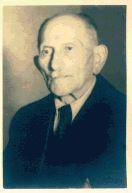
\includegraphics[width=1.5744in,height=2.3063in]{Kurzbiographien-img013.jpg}}
\end{figure}

\bigskip

\textbf{Eigene Werke:}

\begin{itemize}
\item Mirabeau's Gedanken über die Erneuerung des französischen Staatswesens. Karas Halle a. S. 1889 (= Hallesche
Abhandlungen zur neueren Geschichte 23)  
\item Sozialpolitische Seifenblasen. In: Die neue Zeit. Revue des geistigen und öffentlichen Lebens. 15.1896-97, 1. Band
(1897), Heft 18, S. 566–570.  
\item Das Elend des Strafvollzugs. Buchhandlung Vorwärts, Berlin 1905.  
\item Die Wahlrechtsbewegung. In: Sozialistische Monatshefte. 12 = 14(1908), Heft 18/19, S. 1143–1149.  
\item Verfassungswesen und Verfassungskämpfe in Deutschland. Buchhandlung Vorwärts, Berlin 1909.  
\item Die sächsischen Wahlen und die Reichspolitik. In: Sozialistische Monatshefte. 13 = 15(1909), Heft 21, S.
1342–1346.  
\item Nach den sächsischen Wahlen 1909. In: Sozialistische Monatshefte. 13 = 15(1909), Heft 23, S. 1466–1471.  
\item Wahlkampf! Die Sozialdemokratie und ihre Gegner. Kaden, Dresden 1911.  
\item Georg Gradnauer, Robert Schmidt: Die deutsche Volkswirtschaft. Eine Einführung. Buchhandlung Vorwärts, Berlin
1921. 
\item Georg Gradnauer, Rudolf Breitscheid (Hrsg.): Die Vorgeschichte des Weltkrieges. Das Werk des
Untersuchungsausschusses der Verfassunggebenden Deutschen Nationalversammlung und des Deutschen Reichstages. Deutsche
Verlags- Gesellschaft für Politik und Geschichte, Berlin 1919–1930.
\end{itemize}

\bigskip

\textbf{Sekundärliteratur:}

\begin{itemize}
\item E. Herbig: Gradnauer, Georg. In: Geschichte der deutschen Arbeiterbewegung. Biographisches Lexikon. Dietz Verlag,
Berlin 1970, S. 162–163.  
\item Martin Schumacher (Hrsg.): M.d.R. Die Reichstagsabgeordneten der Weimarer Republik in der Zeit des
Nationalsozialismus. Politische Verfolgung, Emigration und Ausbürgerung, 1933–1945. Eine biographische Dokumentation.
3., erheblich erweiterte und überarbeitete Auflage. Droste, Düsseldorf 1994, ISBN 3-7700-5183-1.  
\item Mike Schmeitzner: Georg Gradnauer und die Begründung des Freistaates Sachsen 1918–1920. Parlamentarisierung und
Demokratisierung der sächsischen Revolution. In: Landesgeschichte in Sachsen. Tradition und Innovation. Sächs.
Landeszentrale f. polit. Bildung, Dresden 1997, S. 249–270.  
\item Mike Schmeitzner: Georg Gradnauer. Der Begründer des Freistaates Sachsen (1918–20). In: ders., Andreas Wagner
(Hrsg.): Von Macht und Ohnmacht. Sächsische Ministerpräsidenten im Zeitalter der Extreme 1919–1952. Sax-Verlag, Bucha
2006, ISBN 978-3-934544-75-8, S. 52–88.
\end{itemize}

\bigskip


\bigskip

\textbf{Internetquellen:}

\begin{itemize}
\item \url{http://www.ghetto-theresienstadt.de/pages/g/grandnauerg.htm} 
\item \url{https://de.wikipedia.org/wiki/Georg_Gradnauer} 
\end{itemize}

\bigskip

\textbf{Bildquelle:}

\begin{itemize}
\item \url{http://www.ghetto-theresienstadt.de/images/prominente/Bild89.gif} 
\end{itemize}
\textbf{Fiedrich 'Fritz' Bernhard Eugen Gutmann} [geb. 15.11.1886 in Berlin (Deutsches Reich); gest. 13.04.1944 im
Ghetto Theresienstadt (Tschechoslowakei)] war ein dänischer Bankier, Leiter der Dresdner Bank und Kunstsammler.

\begin{figure}[h]
\centering
\lfbox[margin-top=0.1181in,margin-right=0.1181in,margin-bottom=0.1181in,margin-left=0.1181in,border-style=none,padding=0mm,vertical-align=top,raise=-0.9055in]{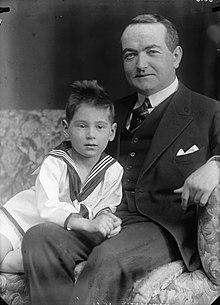
\includegraphics[width=1.5744in,height=2.1839in]{Kurzbiographien-img014.jpg}}
\end{figure}
Er wurde mit seiner Frau Louise (geb. von Landau, in Ausschwitz ermordet) und seinen Kindern Lili und Bernard
(überlebten) am 26.05.43 mit dem Transport XXIV/1 Ez1 in das Ghetto Theresienstadt deportiert. Im Ghetto trug er Kohlen
aus. Seine Gemahlin erteilte trotz des Verbots Englisch-Unterricht. Im Propoganadafilm ist er in der Sequenz
\textit{Konzert} (34) zu sehen. Er wurde am 13.04.1944 im Ghetto Theresienstadt ermordet.


\bigskip

\textbf{Sekundärliteratur:}

\begin{itemize}
\item Anne Webber, {\textquotedbl}Introduction to the Gutmann Sale Catalogue,{\textquotedbl} Christie’s,
{\textquotedbl}Sale 2590: Property from the Gutmann Collection,{\textquotedbl} May 13, 2003 (Amsterdam)
\item {\textquotedbl}Nazis killed Simon Goodman's grandparents and stole their art; new book tells how he got some of it
back{\textquotedbl} in Los Angeles Times, 20 October 2015
\item Lili Gutmann statement, {\textquotedbl}Making a Killing{\textquotedbl} (Part I) (1998; documentary produced by
Anne Webber and executive producer Roy Ackerman).
\end{itemize}

\bigskip

\textbf{Internetquellen:}

\begin{itemize}
\item \url{http://www.ghetto-theresienstadt.de/pages/g/gutmannf.htm} 
\end{itemize}

\bigskip

\textbf{Bildquelle:}

\begin{itemize}
\item
\url{https://en.wikipedia.org/wiki/Friedrich_Gutmann#/media/File:Friedrich_Bernhard_Eugen_Gutmann_met_zoon_Bernhard.jpg}

\end{itemize}
\textbf{Pavel Haas }(auch Paul Haas) [geb. 21.06.1899 in Brünn (Österreich-Ungarn); gest. 17./18.10.1944 im KZ Auschwitz
(Generalgouvernement Polen)] war ein tschechoslowakischer-deutschsprachiger Komponist.

\begin{figure}[h]
\centering
\lfbox[margin-top=0.1181in,margin-right=0.1181in,margin-bottom=0.1181in,margin-left=0.1181in,border-style=none,padding=0mm,vertical-align=top,raise=-0.9055in]{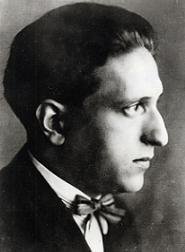
\includegraphics[width=1.5744in,height=2.1484in]{Kurzbiographien-img015.jpg}}
\end{figure}
In den 1930er Jahren schuf er für Filme. 1929 Vorsitzender des Mährischen Komponistenverbands. Ab 1935 war er
Privatlehrer für Musiktheorie und schließlich Musiklehrer an der Hochschule in Brünn und freischaffender Komponist. Er
komponierte Auftragswerke für renommierte Ensembles wie das Mährische Streichquartett und das Mährische Bläserquintett
sowie für den Rundfunk. Am 02.04.1938 wurde die dreiaktige Oper Der Scharlatan (Šarlatán) mit großem Erfolg
uraufgeführt. Dieser Premiere folgten im Frühjahr 1938 bis zum Verbot noch fünf weitere Aufführungen. Nach dem
Einmarsch deutscher Truppen in die Tschechoslowakei wurde die Aufführung seiner Musik verboten und er erhielt
Erwerbsverbot. Er ließ sich von seiner Frau Soňa Jakobson am 13.04.1940, zum Schutz von Ihr und seinen Kindern
scheiden. Am 02.12.1941 wurde er mit dem Transport G-731 in das Ghetto Theresienstadt deportiert. Im Ghetto komponierte
er für die Künstler und Laienchöre. Anlässlich des Besuches des Internationalen Komitee vom Roten Kreuz wurde Haas’
Studie für Streichorchester von Karel Ančerl uraufgeführt. Außer dem Chor mit hebräischem Text Al s{\textasciigrave}fod
! (Klage nicht!) und allegorischer Widerstandsthematik komponierte er für das Streichorchester Karel Ancerls eine
Studie. Karel Berman widmete er Ctyri pisne na slova čínské poezie (Vier Lieder auf Worte aus der chinesischen Poesie).
Im Propoganadafilm ist er in der Sequenz \textit{Konzert} (34) zu sehen. Am 16.10.1944 wurde er nach Auschwitz
deportiert und dort ermordet.


\bigskip

\textbf{Eigene Werke:}

\begin{itemize}
\item vgl. \url{https://de.wikipedia.org/wiki/Pavel_Haas} 
\end{itemize}

\bigskip

\textbf{Sekundärliteratur:}

\begin{itemize}
\item Die Musik in Geschichte und Gegenwart. (MGG) 1 (1949) – 10(1962), Band 5.  
\item Hugo Riemann: Riemann Musiklexikon. 12. Auflage. Band 1, Mainz 1972.  Haas, Paul, Komponist. In: Heribert Sturm:
Biographisches Lexikon zur Geschichte der böhmischen Länder. Herausgegeben im Auftrag des Collegium Carolinum. Band I.
Oldenbourg, München/Wien 1979, ISBN 3-486-49491-0, S. 469.  
\item Jascha Nemtsov: Zur Klaviersuite op. 13 von Pavel Haas. In: Musica Reanimata Mitteilungen. Hrsg. von Musica
Reanimata, Berlin, Nr. 17, Dez. 1995, ISSN 0943-5093, S. 20–23.  
\item Lubomír Peduzzi: Pavel Haas. Leben und Werk des Komponisten (= Musica Reanimata, Förderverein zur Wiederentdeckung
NS-verfolgter Komponisten und ihrer Werke: Verdrängte Musik. Band 9). Übersetzt von Thomas Mandl. von Bockel, Hamburg
1996, ISBN 3-928770-28-4 (Originaltitel: Pavel Haas: Život a dílo skladatele, Brno 1993).  
\item Milan Kuna: Musik an der Grenze des Lebens. Musikerinnen und Musiker aus böhmischen Ländern in
nationalsozialistischen Konzentrationslagern und Gefängnissen. Zweitausendeins, Frankfurt am Main 1998, ISBN
3-86150-260-7.  
\item Jolana Matějková: Hugo Haas. Život je pes. Nakladatelství XYZ, Prag 2005, ISBN 80-7106-724-5.  Louise Mary
O’Sullivan: Selected Performances and Compositions of the Theresienstadt Ghetto (1941–1945) – An Examination of Music,
Memory and Survivance. Department of Music an der National University of Ireland in Maynooth, 2012.  
\item MGG. Kassel 2002.  
\item The New Grove. London 2001.  
\item Uwe Harten: Haas, Paul (Pavel). In: Oesterreichisches Musiklexikon. Online-Ausgabe, Wien 2002 ff., ISBN
3-7001-3077-5; Druckausgabe: Band 2, Verlag der Österreichischen Akademie der Wissenschaften, Wien 2003, ISBN
3-7001-3044-9.  
\item Haas, Paul. In: Österreichisches Biographisches Lexikon 1815–1950 (ÖBL). Band 2, Verlag der Österreichischen
Akademie der Wissenschaften, Wien 1959, S. 118 f. (Direktlinks auf S. 118, S. 119)., ISBN 3-7001-0187-2.
\end{itemize}

\bigskip


\bigskip

\textbf{Internetquellen:}

\begin{itemize}
\item \url{http://www.ghetto-theresienstadt.de/pages/h/haasp.htm} 
\item \url{https://de.wikipedia.org/wiki/Pavel_Haas} 
\end{itemize}

\bigskip

\textbf{Bildquelle:}

\begin{itemize}
\item \url{https://de.wikipedia.org/wiki/Pavel_Haas#/media/Datei:PavelHaas.jpg} 
\end{itemize}
\textbf{Dr. Franz Kahn} [geb. 13.06.1895 in Pilsen (Tschechoslowakei); gest. 04.10.1944 im KZ Auschwitz
(Generalgouvernement Polen)] war ein tschechoslowakischer Zionist, Generalsekretär der zionistischen Organisationen und
Direktor des Büros des zionistischen Kongresses in der Tschechien.

\begin{figure}[h]
\centering
\lfbox[margin-top=0.1181in,margin-right=0.1181in,margin-bottom=0.1181in,margin-left=0.1181in,border-style=none,padding=0mm,vertical-align=top,raise=-0.9055in]{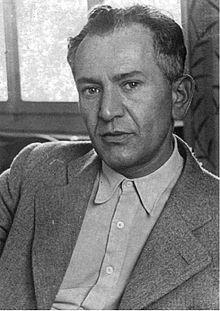
\includegraphics[width=1.5744in,height=2.2236in]{Kurzbiographien-img016.jpg}}
\end{figure}
Er wurde Ende Januar 1943 mit dem Transport Ez 160 in das Ghetto Theresienstadt Seine Frau Olga (geb. Kahnová) folgte
einen Tag später. Im Ghetto übernahm er in der \textit{Kulturabteilung} den Posten des Fachleiters für das
\textit{Vorlesungswesen} mit Schwerpunkt auf Zionismus und Judentum. Im Propoganadafilm ist er in der Sequenz
\textit{Konzert} (34) zu sehen. Am 04.10.1944 wurde er nach Auschwitz deportiert und dort ermordet.


\bigskip

\textbf{Eigene Werke}:

\begin{itemize}
\item Abhandlungen zum internationalen Privatrecht, 1928.
\end{itemize}

\bigskip

\textbf{Sekundärliteratur:}

\begin{itemize}
\item Theresienstadt (Heb., 1947); 
\item Ch. Yahil, Devarim al ha-[1E92?]iyyonut ha-Czechoslovakit (1967).
\item Israel Gutman (Hrsg.): Enzyklopädie des Holocaust – Die Verfolgung und Ermordung der europäischen Juden, Piper
Verlag, München/Zürich 1998, 3 Bände, ISBN 3-492-22700-7. (Eintrag: Kahn, Franz in Band 2, S. 727 f.)  
\item Susanne Blumesberger, Michael Doppelhofer, Gabriele Mauthe: Handbuch österreichischer Autorinnen und Autoren
jüdischer Herkunft 18. bis 20. Jahrhundert. Band 2: J–R. Hrsg. von der Österreichische Nationalbibliothek. Saur,
München 2002, ISBN 3-598-11545-8, S. 626.  
\item Hans G. Adler: Theresienstadt. Das Antlitz einer Zwangsgemeinschaft 1941–1945; Nachwort Jeremy Adler; Wallstein,
Göttingen 2005 ISBN 3-89244-694-6 (Reprint der 2. verb. Auflage Mohr-Siebeck, Tübingen 1960. 1. Auflage ebd. 1955).
\end{itemize}

\bigskip

\textbf{Internetquellen:}

\begin{itemize}
\item \url{http://www.ghetto-theresienstadt.de/pages/k/kahnf.htm} 
\item https://www.holocaust.cz/de/opferdatenbank/opfer/96946-franz-kahn/ ;
\url{https://www.jewishvirtuallibrary.org/kahn-franz} 
\item \url{https://de.wikipedia.org/wiki/Franz_Kahn_(Zionist}) 
\end{itemize}

\bigskip

\textbf{Bildquelle:}

\begin{itemize}
\item \url{https://he.wikipedia.org/wiki/%D7%A4%D7%A8%D7%A0%D7%A5_%D7%A7%D7%90%D7%94%D7%9F} 
\end{itemize}
\textbf{Hans Krása} [geb. 30.11.1899 in Prag (Österreich-Ungarn); gest. 17.10.1944 im KZ Auschwitz (Generalgouvernement
Polen)] war ein tschechoslowakischer-deutschsprachiger Komponist.

\begin{figure}[h]
\centering
\lfbox[margin-top=0.1181in,margin-right=0.1181in,margin-bottom=0.1181in,margin-left=0.1181in,border-style=none,padding=0mm,vertical-align=top,raise=-0.9055in]{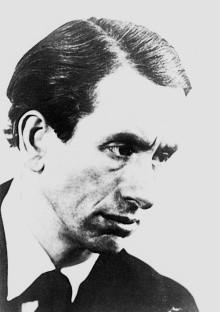
\includegraphics[width=1.5744in,height=2.2354in]{Kurzbiographien-img017.jpg}}
\end{figure}
1921 ersten Erfolg als Komponist. 1933 wurde in Prag seine Oper Verlobung im Traum uraufgeführt. 1938 schrieb Krása die
Kinderoper \textit{Brundibár}. 1941 wurde diese Oper heimlich im jüdischen Waisenhaus in Prag uraufgeführt. Er wurde am
10.08.42 in das Ghetto Theresienstadt deportiert. Im Ghetto heiratete er Eliška Kleinová, um deren Deportation zu
verhindern. Sein \textit{Brundibár} wurde in Theresienstadt über 55-mal aufgeführt. Im Propoganadafilm ist er in der
Sequenz \textit{Konzert} (34 –bei 21:19min) zu sehen. Am 16. Oktober 1944 wurde er nach Auschwitz deportiert und dort
ermordet.


\bigskip

\textbf{Eigene Werke (nur Opern):} 

\begin{itemize}
\item Verlobung im Traum, 1928–1930, nach Dostojewskis Novelle Onkelchens Traum (Bote \& Bock)  
\item Brundibár, Oper für Kinder (zwei Fassungen: Prag 1938, Theresienstadt 1943) (Bote \& Bock)  
\end{itemize}

\bigskip


\bigskip

\textbf{Sekundärliteratur:}

\begin{itemize}
\item Joža Karas: Music in Terezín 1941–1945. Pendragon Press, Stuyvesant NY 1990, ISBN 0-918728-34-7.  
\item Blanka Červinková (Übersetzung: Hana Smolíková): Hans Krása. Leben und Werk. Pfau, Saarbrücken 2005, ISBN
3-89727-305-5.  
\item Inken Meents: Hans Krása. In: Lexikon verfolgter Musiker und Musikerinnen der NS-Zeit. Hrsgg. von Claudia Maurer
Zenck, Peter Petersen und Sophie Fetthauer, Hamburg 2009 Online.
\end{itemize}

\bigskip


\bigskip

\textbf{Internetquellen:}

\begin{itemize}
\item \url{http://www.ghetto-theresienstadt.de/pages/k/krasah.htm} 
\item \url{https://de.wikipedia.org/wiki/Hans_Kr%C3%A1sa} 
\end{itemize}

\bigskip

\textbf{Bildquelle:}

\begin{itemize}
\item \url{https://de.wikipedia.org/wiki/Datei:Hans_Kr%C3%A1sa_(1899-1944).jpg} 
\end{itemize}
\textbf{Dr. Karl Loewenstein} (auch Karl Loesten beziehungsweise Lowen oder Levensteen) [geb. 02.05.1887 in Siegen
(Deutsches Reich); gest. 29.05.1905 in Bad Neuenahr-Ahrweiler (Bundesrepublik Deutschland)] war ein deutscher
Privatbankdirektor. 

Konvertierte 1919 zum evangelischen Glauben. 1924-1941 Bankier und Direktor des Bankhauses Busse \& Co. Er stand der
\textit{Bekennenden Kirche} nahe und erregte so das Missfallen der Nationalsozialisten. Im November 1941 verhaftet und
in das Ghetto Minsk deportiert. Er wurde aufgrund einer Intervention des Generalkommissars für Weißrussland Wilhelm
Kube mit dem Transport Ez 50 in das Ghetto Theresienstadt deportiert. Im Ghetto war er Leiter der
\textit{Sicherheitswesens der jüdischen Selbstverwaltung}. Er hatte damit nach dem Judenältesten die wichtigste
Position im Ghetto inne. Er organisierte die \textit{Feuerwehr},eine \textit{Detektivabteilung} und die
\textit{Wirtschaftsprüfstelle} und andere Einrichtungen der \textit{Ghettowache}. Er vermittelte zwischen dem
Lagerkommandant und SS einerseits und den Häftlingen des Ghettos andererseits in einer Vielzahl von oft auch heiklen
Fällen. Im Propoganadafilm ist er in der Sequenz Konzert (34) zu sehen. Er wurde am späten Abend des 08.05.1945 in
Theresienstadt durch die Rote Armee befreit. 


\bigskip

\textbf{Eigene Werke:}

\begin{itemize}
\item Aus der Hölle Minsk in das ‚Paradies‘ Theresienstadt. Typoskript im Archiv des Leo Baeck Instituts, New York City
(Digitalisat beim Center for Jewish History)  
\item Minsk. Im Lager der deutschen Juden. Bonn 1961 (auch: Minsk – Im Lager der deutschen Juden. In: Beilage zur
Wochenzeitschrift Das Parlament. B 45/46 vom 7. November 1956, S. 706–718) (= 1. Teil von Aus der Hölle Minsk ...)  
\item Korrespondenz mit H.G. Adler, Nachlass Adler, Deutsches Literaturarchiv Marbach.  Seine Ermittlungen vor dem
Volksgericht Litoměřice, Archiv des tschechischen Innenministeriums. ;
https://collections.jewishmuseum.cz/index.php/Browse/modifyCriteria/facet/people\_facet/id/22733/mod\_id/0 
\end{itemize}

\bigskip

\textbf{Sekundärliteratur:}

\begin{itemize}
\item Axel Feuß: Das Theresienstadt-Konvolut. Altonaer Museum in Hamburg, Dölling und Galitz Verlag, Hamburg/München
2002, ISBN 3-935549-22-9.
\end{itemize}

\bigskip


\bigskip

\textbf{Internetquellen:}

\begin{itemize}
\item \url{http://www.ghetto-theresienstadt.de/pages/l/loewensteink.htm} 
\item \url{https://de.wikipedia.org/wiki/Karl_Loewenstein_(Bankier}) 
\end{itemize}

\bigskip

\textbf{Dr. Leo Löwenstein} [geb. 08.02.1879 in Aachen (Deutsches Reich); gest. 13.11.1956 in (Israel)] war ein
deutscher Physiker und Chemiker.

Er war Besitzer eines Laboratoriums für Schädlingsbekämpfung, machte kriegsnützliche Erfindungenund arbeitete mit der
Reichswehr während und nach dem Ersten Weltkrieg zusammen. Er meldete über 20 Patente an, ließ sie jedoch aus
patriotischen Gründen patentrechtlich nicht schützen. 1924 entwickelte er ein Verfahren zur großtechnischen Produktion
von Wasserstoffperoxid (Riedel–Löwenstein–Verfahren). Nach der Reichspogromnacht blieb er als Jude vorerst wegen seines
Ansehens im Reichswehrministerium unbehelligt. Nach Zwangsarbeitsdiensten wurde er 1943 mit seiner Frau mit dem
Transport I/99 in das Ghetto Theresienstadt deportiert. Seine Rolle im Ghetto ist unbekannt. Im Propoganadafilm ist er
in der Sequenz \textit{Konzert} (34) zu sehen. Er wurde am späten Abend des 08.05.1945 in Theresienstadt durch die Rote
Armee befreit. 


\bigskip

\textbf{Eigene Werke:}

\begin{itemize}
\item Beiträge zur Messung von Dissociationen bei hohen Temperaturen. Göttingen: Dieterich 1905, zugl. Göttingen, Univ.,
Diss., 1905
\end{itemize}

\bigskip

\textbf{Sekundärliteratur:}

\begin{itemize}
\item Franz Menges: Löwenstein, Leo. In: Neue Deutsche Biographie (NDB). Band 15, Duncker \& Humblot, Berlin 1987, ISBN
3-428-00196-6, S. 106 f. (Digitalisat).  
\item John F. Oppenheimer (Red.) u. a.: Lexikon des Judentums. 2. Auflage. Bertelsmann Lexikon Verlag, Gütersloh u. a.
1971, ISBN 3-570-05964-2, Sp. 445.  
\item Günter Nagel: Erfinder, Industriemanager, jüdischer Offizier und Politiker – Das Lebenswerk des Dr. Leo
Löwenstein. In: Jahrbuch für brandenburgische Landesgeschichte, 68. Band (2017), S. 181–224
\end{itemize}

\bigskip


\bigskip

\textbf{Internetquellen:}

\begin{itemize}
\item \url{http://www.ghetto-theresienstadt.de/pages/l/loewensteinl.htm} 
\item \url{https://de.wikipedia.org/wiki/Leo_L%C3%B6wenstein} 
\end{itemize}

\bigskip


\bigskip

\textbf{Robert Mandler} [geb. 04.05.1896 in Wien (Österreich-Ungarn); gest. 30.10.1944 im KZ Auschwitz
(Generalgouvernement Polen)] war ein österreichischer Geschäftsmann und Funktionär bei der Jüdischen Kultusgemeinde in
Prag.

\begin{figure}[h]
\centering
\lfbox[margin-top=0.1181in,margin-right=0.1181in,margin-bottom=0.1181in,margin-left=0.1181in,border-style=none,padding=0mm,vertical-align=top,raise=-0.9055in]{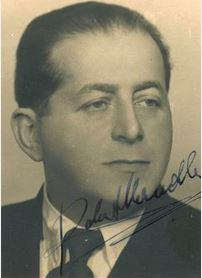
\includegraphics[width=1.5744in,height=2.1689in]{Kurzbiographien-img018.jpg}}
\end{figure}
Er leitete in Prag das, im März 1939 gegründete Transportbüro Jüdische Emigrationshilfe. Ab 1939/1940 arbeitete er im
Auswanderungsamt als Verbindungsmann zur SS. Er war Leiter der Transportabteilung der Prager Jüdischen Kultusgemeinde.
Bei den ins Ghetto Theresienstadt Deportierten waren er und seine Kollegen nach Angaben von H. G. Adler verhasst und
wurden \textit{Der Zirkus} genannt..

Er wurden mit seiner Frau Martha, (geb. Fischer, am 30.01.1943 in Theresienstadt ermordet) und seinem Kindern Rita (geb.
1923, am 30.10.1944 im KZ Auschwitz ermordet) und Hertha (1921-2009) am 29.01.43 mit dem Transport Ez-St\_50 in das
Ghetto Theresienstadt deportiert. Im Ghetto war er Leiter eine Abteilung der \textit{Ghettowache} und Stellvertreter
des Leiters des Sicherheitswesens Karl Loewenstein ernannt. Er hatte eine besondere Rolle bei der Zählung der etwa
40.000 Insassen des Ghettos Theresienstadt im nahegelegenen \textit{Bauschowitzer Kessel} am 11. 11.1943, weil er sich
genau wie der Kommandant des Lagers, verzählte. Das bedeutete für die Insassen, die den ganzen Tag unter
Maschinengewehrbewachung in dem Talkessel ausharren mussten, zusätzliche Qualen. Im Propoganadafilm ist er in der
\textit{Sequenz} Konzert (34) zu sehen.


\bigskip

\textbf{Sekundärliteratur:}

\begin{itemize}
\item William R. Perl: Operation action: rescue from the Holocaust, Frederick Ungar Publishing Corporation, New York
1983.
\end{itemize}

\bigskip

\textbf{Internetquellen:}

\begin{itemize}
\item \url{http://www.ghetto-theresienstadt.de/pages/m/mandlerr.htm} 
\item \url{https://www.holocaust.cz/de/opferdatenbank/opfer/108575-robert-mandler/} ;
\url{https://web.archive.org/web/20120310044905/http://www.lettertothestars.at/lastwitnesses_pers.php?uid=1087} 
\item \url{https://de.wikipedia.org/wiki/Robert_Mandler} 
\end{itemize}

\bigskip

\textbf{Bildquelle:}

\begin{itemize}
\item \url{https://www.holocaust.cz/de/opferdatenbank/opfer/108575-robert-mandler/} 
\end{itemize}
\textbf{Carl Meinhard} (auch Karl Meinhardt) [geb. 28.11.1875 in Iglau (Österreich-Ungarn); gest. 12.02.1949 in Buenos
Aires (Brasilien)] war ein österreichischer Schauspieler, Theaterdirektor.

\begin{figure}[h]
\centering
\lfbox[margin-top=0.1181in,margin-right=0.1181in,margin-bottom=0.1181in,margin-left=0.1181in,border-style=none,padding=0mm,vertical-align=top,raise=-0.9055in]{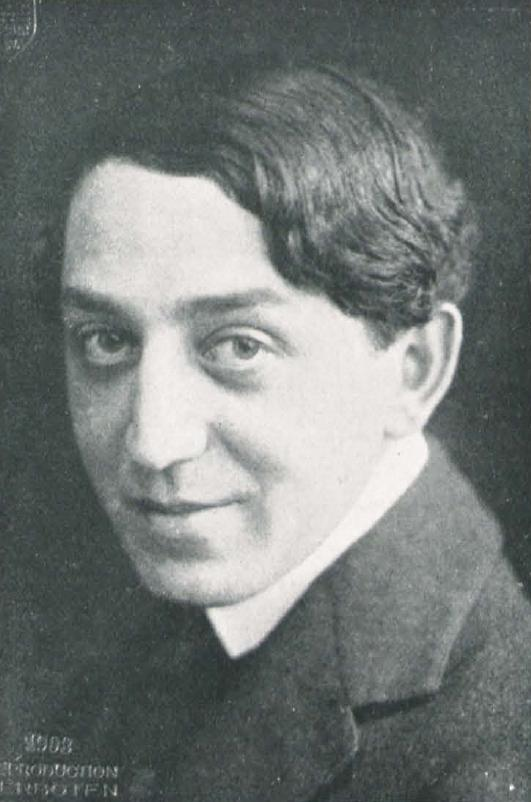
\includegraphics[width=1.5744in,height=2.3772in]{Kurzbiographien-img019.jpg}}
\end{figure}
Zwischen 1918 und 1933 wirkte er in mehreren Filmen mit (z.B. bei der Verfilmung von Emil und die Detektive). Floh 1933
nach Prag. 1936 wurde er nach Wien geholt, um in den Aufsichtsrat der Filmproduktionsfirma Sascha-Messter Filmfabrik
einzutreten. Floh Ende Mai 1938 erneut nach Prag. Er wurde am 24.10.42 in das Ghetto Theresienstadt deportiert. Seine
Rolle im Ghetto ist unbekannt. Im Propoganadafilm ist er in der \textit{Sequenz} Konzert (34) zu sehen. Er wurde am
späten Abend des 08.05.1945 in Theresienstadt durch die Rote Armee befreit.


\bigskip

\textbf{Eigene Werke:}

\begin{itemize}
\item Die wunderlichen Geschichten des Kapellmeisters Kreisler : Phantast. Melodram nach E. T. A. Hoffmanns Leben und
Erzählungen ; Musik mit teilw. Benutzung von Motiven aus Hoffmanns {\textquotedbl}Undine{\textquotedbl} und Mozarts
{\textquotedbl}Don Juan{\textquotedbl} von E. N. von Rezniček. Text von Carl Meinhard; Rudolf Bernauer. Berlin : E.
Reiss, 1922 ; Filmographie:  1918: Mr. Wu  1919: Rausch  1927: Colonialskandal (Liebe im Rausch)  1932: Trenck  1932:
Unheimliche Geschichten  1932: Quick
\end{itemize}

\bigskip

\textbf{Sekundärliteratur:}

\begin{itemize}
\item Joseph Walk (Hrsg.): Kurzbiographien zur Geschichte der Juden 1918–1945. Herausgegeben vom Leo Baeck Institute,
Jerusalem. Saur, München u. a. 1988, ISBN 3-598-10477-4.  
\item Kay Weniger: Zwischen Bühne und Baracke. Lexikon der verfolgten Theater-, Film- und Musikkünstler 1933 bis 1945.
Mit einem Geleitwort von Paul Spiegel. Metropol, Berlin 2008, ISBN 978-3-938690-10-9, S. 244.  
\item Kay Weniger: 'Es wird im Leben dir mehr genommen als gegeben …'. Lexikon der aus Deutschland und Österreich
emigrierten Filmschaffenden 1933 bis 1945. Eine Gesamtübersicht. S. 344 f., ACABUS-Verlag, Hamburg 2011, ISBN
978-3-86282-049-8
\end{itemize}

\bigskip


\bigskip

\textbf{Internetquellen:}

\begin{itemize}
\item \url{https://de.wikipedia.org/wiki/Carl_Meinhard} 
\end{itemize}

\bigskip

\textbf{Bildquelle:}

\begin{itemize}
\item
\href{https://upload.wikimedia.org/wikipedia/commons/0/01/Carl_Meinhard_(BerlLeben_1908-09).jpg}{https://upload.wikimedia.org/wikipedia/commons/0/01/Carl\_Meinhard\_\%28BerlLeben\_1908-09\%29.jpg}

\end{itemize}
\textbf{Dr. Alfred Meissner} (auch Alfréd) [geb. 10.04.1871 in Jungbunzlau (Mladá Boleslav ) (Tschecheslowakei); gest.
29.09.1950 in Prag (Tschechoslowakei)] war ein tschechoslowakischer Jurist, Politiker, Justizminister.

\begin{figure}[h]
\centering
\lfbox[margin-top=0.1181in,margin-right=0.1181in,margin-bottom=0.1181in,margin-left=0.1181in,border-style=none,padding=0mm,vertical-align=top,raise=-0.9055in]{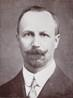
\includegraphics[width=1.5744in,height=2.1134in]{Kurzbiographien-img020.jpg}}
\end{figure}
Nach Gründung der Tschechoslowakei 1918 gehörte er bis 1939 der Prager Nationalversammlung an. 1920 und 1929-1934 war er
Justizminister und 1934/1935 Minister für soziale Fürsorge. Er wurde mit seiner Rosa (geb. Sommer) und seinen 3 Kindern
am 30.01.42 mit dem Transport V 280 in das Ghetto Theresienstadt deportiert. Im Ghetto war er Leiter
\textit{Verlassenschaftsabteilung} am \textit{Ghettogericht} und Mitglied Ältestenrat unter Benjamin Murmelstein. Er
war Mitunterzeichner des Aufrufes des Ältestenrates an die befreiten Mithäftlinge vom 6. Mai 1945, in dem die Übernahme
des Ghettos nach Ende des Zweiten Weltkrieges und damit die Befreiung vom Nationalsozialismus durch ein Internationales
Komitee vom Roten Kreuz mitgeteilt wurde. Er wurde am späten Abend des 08.05.1945 in Theresienstadt durch die Rote
Armee befreit. 


\bigskip

\textbf{Eigene Werke:}

\begin{itemize}
\item Urazové pojištění dělnické dle práva rakouského ... sepsali -{}-{}- a Leo Winter (Die Arbeiterunfallversicherung)
(boh.) V Praze 1904  
\item Jak se volí do obcí v Čechách (mimo Prahu a Liberec.) (Wie in Böhmen in die Gemeinden gewählt wird.) Dělnická
knihtiskárna v Praze 1909  
\item Nároky vdov a sirotků po padlých vojínech. (Ansprüche der Witwen und Waisen der im Kriege gefallenen Soldaten.)
Sveceny V Praze 1914
\item Hlas českého socialního demokrata o krajském zřízení a národnostní autonomii. (Die Stimme des tschechischen
Sozialdemokraten über die Verordnung der Kreiseinteilung und die Volksautonomie.) (boh.) Sveceny V Praze 1916
\item Die Verwaltungsreform in Österreich, um 1917  Kommentar zur neuen tschechoslowakischen Gemeindewahlordnung, A.
Sveceny, Prag um 1924  Die Lage der kleinen Landwirte nach der Bodenreform, A. Sveceny, Prag um 1929
\end{itemize}

\bigskip

\textbf{Sekundärliteratur:}

\begin{itemize}
\item Axel Feuß: Das Theresienstadt-Konvolut, Altonaer Museum in Hamburg, Dölling und Galitz Verlag, Hamburg/München
2002, ISBN 3-935549-22-9  
\item J. Cvetler: Meissner, Alfred. In: Österreichisches Biographisches Lexikon 1815–1950 (ÖBL). Band 6, Verlag der
Österreichischen Akademie der Wissenschaften, Wien 1975, ISBN 3-7001-0128-7, S. 200 f. 
\item  Heribert Sturm (Hrsg.): Biographisches Lexikon zur Geschichte der böhmischen Länder, herausgegeben im Auftrag des
Collegium Carolinum (Institut), Band II, R. Oldenbourg Verlag München 1984, ISBN 3 486 52551 4, Seite 631  S. Winiger:
Große Jüdische National-Biographie
\end{itemize}

\bigskip


\bigskip

\textbf{Internetquellen:}

\url{http://www.ghetto-theresienstadt.de/pages/m/meissneral.htm} 

\url{https://de.wikipedia.org/wiki/Alfred_Meissner} 


\bigskip

\textbf{Bildquelle:}

\url{https://upload.wikimedia.org/wikipedia/commons/b/b1/Alfr%C3%A9d_Meissner.jpg} 

\textbf{Léon Meyer} [geb. 11.09.1868 in Le Havre (Frankreich); gest. 22.01.1948 in Paris (Frankreich)] war ein
französischer Politiker, Minister, Bürgermeister.

\begin{figure}[h]
\centering
\lfbox[margin-top=0.1181in,margin-right=0.1181in,margin-bottom=0.1181in,margin-left=0.1181in,border-style=none,padding=0mm,vertical-align=top,raise=-0.9055in]{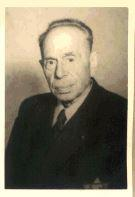
\includegraphics[width=1.5744in,height=2.2984in]{Kurzbiographien-img021.jpg}}
\end{figure}
1889 gründete er 1889 eine Kaffee-Import-Firma. 1902-1919 Präsident der Vereinigung der Kaffeeimporteure. 1912-1919
Stadtrat von Le Havre und 1919-1941 dortiger Bürgermeister. Als Abgeordneter der Radikal-Sozialistischen Partei war er
1923-1940 Mitglied der französischen Deputiertenkammer. 1924 und 1932-1933 Handelsmarine-Minister. 1931
Handelsminister. 1937 Vizepräsident der Kommission für auswärtige Angelegenheiten der Deputiertenkammer. Spätestens
1944 in das Aufenthaltslager Bergen-Belsen deportiert. Von dort wurde er mit seiner Frau Susanne und seiner Tochter am
12.07.42 in das Ghetto Theresienstadt deportiert. Seine Rolle im Ghetto ist unbekannt. Er wurde am späten Abend des
08.05.1945 in Theresienstadt durch die Rote Armee befreit. 


\bigskip

\textbf{Sekundärliteratur:}

\begin{itemize}
\item Axel Feuß: Das Theresienstadt-Konvolut, Altonaer Museum in Hamburg, Dölling und Galitz Verlag, Hamburg/München
2002, ISBN 3-935549-22-9  Meyer, Léon, in: Encyclopaedia Judaica, 1971, Band 11, Sp. 1464
\end{itemize}

\bigskip

\textbf{Internetquellen:}

\begin{itemize}
\item \url{http://www.ghetto-theresienstadt.de/pages/m/meyerl.htm} 
\item \url{https://de.wikipedia.org/wiki/L%C3%A9on_Meyer} 
\end{itemize}

\bigskip

\textbf{Bildquelle:}

\begin{itemize}
\item \url{http://www.ghetto-theresienstadt.de/images/prominente/Bild61.gif} 
\end{itemize}
\textbf{Dr. Owe Meyer} (auch Ove) [geb. 16.10.1885 in Kopenhagen (Dänemark); gest. nach 1945] war ein dänischer
Diplom-Ingenieur, Direktor einer großen Accumulatorenfabrik in Kopenhagen, Leiter des Exportbüros des dänischen
Industrierates und Direktor der Kunstporzellanfabrik Bing und Groendahl.

\begin{figure}[h]
\centering
\lfbox[margin-top=0.1181in,margin-right=0.1181in,margin-bottom=0.1181in,margin-left=0.1181in,border-style=none,padding=0mm,vertical-align=top,raise=-0.9055in]{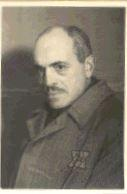
\includegraphics[width=1.5744in,height=2.4047in]{Kurzbiographien-img022.jpg}}
\end{figure}
Er wurde am 06.10.43 in das Ghetto Theresienstadt deportiert. Seine Rolle im Ghetto ist unbekannt Im Propoganadafilm ist
er zu sehen in der Sequenz Konzert (34) zu sehen. Er wurde am späten Abend des 08.05.1945 in Theresienstadt durch die
Rote Armee unbekannt. 


\bigskip

\textbf{Internetquellen:}

\begin{itemize}
\item \url{http://www.ghetto-theresienstadt.de/pages/m/meyero.htm} 
\end{itemize}

\bigskip

\textbf{Bildquelle:}

\begin{itemize}
\item \url{http://www.ghetto-theresienstadt.de/images/prominente/Bild60.gif} 
\end{itemize}
\textbf{Prof. Dr. Alfred Philippson }[geb. 01.01.1864 in Bonn (Deutsches Reich); gest. 28.03.1953 in Bonn
(Bundesrepublik Deutschland)] war ein deutscher Geograph.

\begin{figure}[h]
\centering
\lfbox[margin-top=0.1181in,margin-right=0.1181in,margin-bottom=0.1181in,margin-left=0.1181in,border-style=none,padding=0mm,vertical-align=top,raise=-0.9055in]{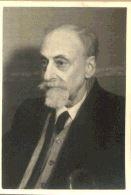
\includegraphics[width=1.5744in,height=2.3417in]{Kurzbiographien-img023.jpg}}
\end{figure}
1892-1933 in Bonn als Privatdozent/Professor der Geographie. 1933 erhielt er Lehrverbot. 1938 wurde ihm der Reisepass
entzogen. Im Juli 1941 beschlagnahmte die Bonner Gestapo sein Haus und wies ihm mit seiner Frau Margarete und seiner
Tochter Dora eine kleine Wohnung im Haus des jüdischen Rechtsanwaltes Wollstein zu. 1941/42 bemühte er sich um eine
Einreisebewilligung für die Schweiz. Er wurde am 08.06.1942 mit seiner Frau Margarethe (geb. Kirchberger) und der
Tochter Dora mit dem Transport 544-III/1 in das Ghetto Theresienstadt deportiert. Im Ghetto schrieb vom Oktober 1942 an
iseine Lebenserinnerungen \textit{Wie ich zum Geographen wurde }nieder. Im Propoganadafilm ist er zu sehen in der
Sequenz \textit{Vortrag} (33) zu sehen. Er und seine Familie wurde am späten Abend des 08.05.1945 in Theresienstadt
durch die Rote Armee befreit und kehrten nach Bonn zurück, wo er seine Publikationstätigkeit wieder aufnahm und im
November 1945 auch eine erneuerte Lehrbefugnis erhielt . 


\bigskip

\textbf{Eigene Werke (Auswahl):}

\begin{itemize}
\item Die griechischen Landschaften. Vier Bände, Klostermann, Frankfurt am Main 1950–1959.  
\item Das Mittelmeergebiet, seine geographische und kulturelle Eigenart. 1904, 4. Auflage 1922.  
\item Grundzüge der Allgemeinen Geographie. Drei Bände, 1920–1924.  
\item Wie ich zum Geographen wurde. 1942/1996, ISBN 3-416-02620-9.  
\item Land und See der Griechen. 1946.  
\item Das Klima Griechenlands. 1948.  
\item Handbuch der regionalen Geologie: Kleinasien. In: Handbuch der regionalen Geologie, Band 22, 1968.
\end{itemize}

\bigskip

\textbf{Sekundärliteratur:}

\begin{itemize}
\item Johanna Philippson: The Philippsons, a German-Jewish Family 1775–1933. In: Leo Baeck Institute Yearbook. 7 (1962),
95–118 (englisch).  
\item Astrid Mehmel: „Wie ich zum Geographen wurde“ - Aspekte zum Leben Alfred Philippsons. In: Geographische
Zeitschrift 82, 1994, S. 116–132.  
\item Astrid Mehmel, Claudia Hermes: Alfred Philippson - Lebenserinnerungen eines Geographen - Hinwegsehen über sein
Judentum. In: Aufbau New York LX 16 vom 5. August 1994, S. 4–5.  
\item Astrid Mehmel: Deutsche Revisionspolitik in der Geographie nach dem Ersten Weltkrieg. In: Geographische Rundschau
9, September 1995, S. 498–505.  
\item Hans Böhm, Astrid Mehmel: Alfred Philippson: Wie ich zum Geographen wurde. Aufgezeichnet im Konzentrationslager
Theresienstadt zwischen 1942 und 1945. Herausgegeben und kommentiert von Hans Böhm und Astrid Mehmel. Bonn 1996.
Erweiterte Auflage Bonn 2000.  
\item B. Brandenburg, Astrid Mehmel: Margarete Kirchberger, verheiratete Philippson. In: 100 Jahre Frauenstudium: Frauen
der Rheinischen Friedrich-Wilhelms-Universität Bonn. Herausgegeben von Annette Kuhn u. a. Dortmund 1996, S. 156–159. 
\item Astrid Mehmel: Dora Philippson. In: 100 Jahre Frauenstudium: Frauen der Rheinischen Friedrich-Wilhelms-Universität
Bonn. Herausgegeben von Annette Kuhn u. a. Dortmund 1996, S. 200–204.  
\item Hans Böhm: Alfred Philippsons Begegnungen mit Griechenland 1887-1934. In: Ernst Trapp (Hrsg.): 3000 Jahre
Griechische Kultur. St. Augustin 1997, S. 145–171.  
\item Astrid Mehmel: Alfred Philippson (1. Januar 1864-28. März 1953) - ein deutscher Geograph. In: Aschkenas.
Zeitschrift für Geschichte und Kultur der Juden. Bd. 8, Heft 2, 1998, S. 353–379.  
\item Astrid Mehmel: Philippson, Alfred. In: Neue Deutsche Biographie (NDB). Band 20, Duncker \& Humblot, Berlin 2001,
ISBN 3-428-00201-6, S. 399 f. (Digitalisat).  
\item Sabine Richter: Wissenschaftliche Nachlässe im Archiv des Geographischen Instituts der Universität Bonn.
Findbücher zu den Nachlässen von Carl Troll und Alfred Philippson. Asgard, Sankt Augustin 2004. (= Colloquium
Geographicum 27) ISBN 3-537-87427-8  
\item Josef Niesen: Bonner Personenlexikon. Bouvier, Bonn 2007, ISBN 978-3-416-03159-2, S. ?
\end{itemize}

\bigskip


\bigskip

\textbf{Internetquellen:}

\begin{itemize}
\item \url{http://www.ghetto-theresienstadt.de/pages/p/philippsona.htm} 
\item \url{https://de.wikipedia.org/wiki/Alfred_Philippson} 
\end{itemize}

\bigskip

\textbf{Bildquelle:}

\begin{itemize}
\item \url{http://www.ghetto-theresienstadt.de/images/prominente/Bild46.gif} 
\end{itemize}
\textbf{Rudolf Saudek }[geb. 20.10.1880 in Kolín (Böhmen); gest. 19.07.1965 in Prag (Tschechoslowakei)] war ein
tschechisch-deutscher Bildhauer, Grafiker und Professor.

\begin{figure}[h]
\centering
\lfbox[margin-top=0.1181in,margin-right=0.1181in,margin-bottom=0.1181in,margin-left=0.1181in,border-style=none,padding=0mm,vertical-align=top,raise=-0.9055in]{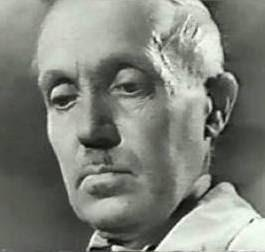
\includegraphics[width=1.5744in,height=1.4953in]{Kurzbiographien-img024.jpg}}
\end{figure}
Seit 1910 als freischaffender Künstler in Leipzig. Überarbeitete 1910 Totenmaske Friedrich Nietzsches. Im Auftrage von
Leipziger Verlegern schuf er 1916 für die Deutsche Bücherei Büsten von Arthur Schopenhauer, Friedrich Nietzsche und
Philalethes. Er arbeitete auch für das Schauspielhaus. Als Beispiel für sein grafisches Schaffen stehen Radierungen zu
Dantes Göttlicher Komödie. 1935 Berufsverbot. 1938 zog er von Leipzig nach Prag. Er wurde 1942 (genaues Datum
unbekannt) in das Ghetto Theresienstadt deportiert. Im Ghetto führte er sein künstlerisches Schaffen fort. Im
Propoganadafilm, in der Sequenz \textit{In der Töpferei} (28) sieht man Rudolf Saudek bei der Arbeit an einer Statue
(11:45min-12:20min), dann seines Hammers und anderer Materialien (11:48min-11:52min). Er wohnt dem \textit{Konzert} (34
- 20:51min) bei. Ob er auch beim Fußballspiel (30) anwesend war, ist umstritten. Er wurde am späten Abend des
08.05.1945 in Theresienstadt durch die Rote Armee befreit. Er kehrte nach Prag zurück, wo er bis zu seinem Tod als
Künstler und Professor an der Akademie der Bildenden Künste Prag tätig war.


\bigskip

\textbf{Sekundärliteratur:}

\begin{itemize}
\item Julius Zeitler: Rudolph Saudek. Mit 9 Abbildungen nach Plastiken des Künstlers. In: Reclams Universum, 34,1
(1918), S. 761–764.  
\item Horst Riedel: Stadtlexikon Leipzig von A bis Z. Pro Leipzig, Leipzig 2005, ISBN 3-936508-03-8, S. 520.
\end{itemize}

\bigskip

\textbf{Internetquellen:}

\begin{itemize}
\item \url{http://blog.despinoza.nl/log/rudolf-saudek-1880-1965-maakte-een-spinozabeeld.html} 
\item Saudek, Rudolf. In: Leipziger Biographie. Abgerufen am 27. April 2015. Rudolf Saudek (1880–1965) maakte een
Spinozabeeld (niederländisch, mit zahlreichen Abbildungen seiner Werke).
\item \url{https://de.wikipedia.org/wiki/Rudolf_Saudek} 
\end{itemize}

\bigskip

\textbf{Bildquelle:}

\begin{itemize}
\item \url{http://blog.despinoza.nl/log/rudolf-saudek-1880-1965-maakte-een-spinozabeeld.html} 
\end{itemize}
\textbf{Ida Franziska 'Franzi' Schneidhuber} (geb. Wassermann) [geb. 07.06.1892 in München (Deutsches Reich); gest. nach
1945] war die Ehefrau von August Schneidhuber, dem SA-Obergruppenführer und Polizeichef von München, der Chef der SA in
Bayern und Mitglied des Deutschen Reichstages war (gest. 1934).

\begin{figure}[h]
\centering
\lfbox[margin-top=0.1181in,margin-right=0.1181in,margin-bottom=0.1181in,margin-left=0.1181in,border-style=none,padding=0mm,vertical-align=top,raise=-0.9055in]{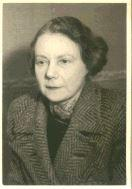
\includegraphics[width=1.5744in,height=2.2555in]{Kurzbiographien-img025.jpg}}
\end{figure}
Sie wurden am 30.07.1942 mit dem Transport II/20-968 in das Ghetto Theresienstadt deportiert. Ihre Rolle im Ghetto ist
unbekannt. Im Propoganadafilm ist sie in den Sequenzen \textit{Freilichtvarietee} (22) und \textit{Vortrag} (32) zu
sehen. Sie wurde am späten Abend des 08.05.1945 in Theresienstadt durch die Rote Armee befreit. Über ihr weiteres Leben
ist nichts bekannt.


\bigskip

\textbf{Internetquellen:}

\begin{itemize}
\item \url{http://www.ghetto-theresienstadt.de/pages/s/schneidhuberi.htm} 
\end{itemize}

\bigskip

\textbf{Bildquelle:}

\begin{itemize}
\item \url{http://www.ghetto-theresienstadt.de/images/prominente/Bild31.gif} 
\end{itemize}
\textbf{Emil Sommer} (auch Emil Samule von Sommer) [geb. 19.11.1869 in Dorna-Watra (Bukowina); gest. 10.04.1947 in
Danvers (Massachusetts, USA)] war ein österreichisch-deutscher Offizier und Generalmajor.

\begin{figure}[h]
\centering
\lfbox[margin-top=0.1181in,margin-right=0.1181in,margin-bottom=0.1181in,margin-left=0.1181in,border-style=none,padding=0mm,vertical-align=top,raise=-0.9055in]{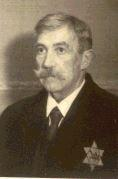
\includegraphics[width=1.5744in,height=2.389in]{Kurzbiographien-img026.jpg}}
\end{figure}
Ab 1889 Berufsoffizier und im Ersten Weltkrieg Bataillonskommandeur. 1922 war er Leiter der militärischen Eroberung des
Burgenlandes und wurde daraufhin Generalmajor. 1924 Ruhestand. 1932 gründete er den Bund jüdischer Frontsoldaten (BJF),
spaltete sich 1934 von diesem ab und gründete die Legitimistischen jüdischen Frontkämpfer (LJF). Er wurde mit seiner
Frau Anna (geb. Mittler) und seiner Tochter Erika (1909–1988) und dem Sohn Anton (1911–1992) am 12.09.42 mit dem
Transport 690-IV/10 in das Ghetto Theresienstadt deportiert. Seine Rolle im Ghetto ist unbekannt. Er wurde am späten
Abend des 08.05.1945 in Theresienstadt durch die Rote Armee befreit. 


\bigskip

\textbf{Sekundärliteratur:}

\begin{itemize}
\item M. Senekowitsch: Sommer Emil. In: Österreichisches Biographisches Lexikon 1815–1950 (ÖBL). Band 12, Verlag der
Österreichischen Akademie der Wissenschaften, Wien 2001–2005, ISBN 3-7001-3580-7, S. 412.  
\item Marthi Pritzker-Ehrlich und Andreas Pritzker: Gestörte Bürgerlichkeit. Zeugnisse einer jüdisch-christlichen
Familie in Briefen, Dokumenten und Bildern. Munda, Brugg 2007, Band 1 (Zeitraum 1802–1937), ISBN 978-3-9523161-0-8;
Band 2 (Zeitraum 1938–1948), ISBN 978-3-9523161-1-5.
\end{itemize}

\bigskip

\textbf{Internetquellen:}

\begin{itemize}
\item \url{http://www.ghetto-theresienstadt.de/pages/s/sommere.htm} 
\item \url{https://de.wikipedia.org/wiki/Emil_Sommer_(General}) 
\end{itemize}

\bigskip

\textbf{Bildquelle:}

\begin{itemize}
\item \url{http://www.ghetto-theresienstadt.de/images/prominente/Bild24.gif} 
\end{itemize}
\textbf{Joseph 'Jo' Eduard Adolf Spier} [geb. 26.06.1900 in Zutphen (Niederlande); gest. 21.05.1978 in Santa Fe (New
Mexiko, USA)] war ein niederländischer Künstler und Illustrator.

\begin{figure}[h]
\centering
\lfbox[margin-top=0.1181in,margin-right=0.1181in,margin-bottom=0.1181in,margin-left=0.1181in,border-style=none,padding=0mm,vertical-align=top,raise=-0.9055in]{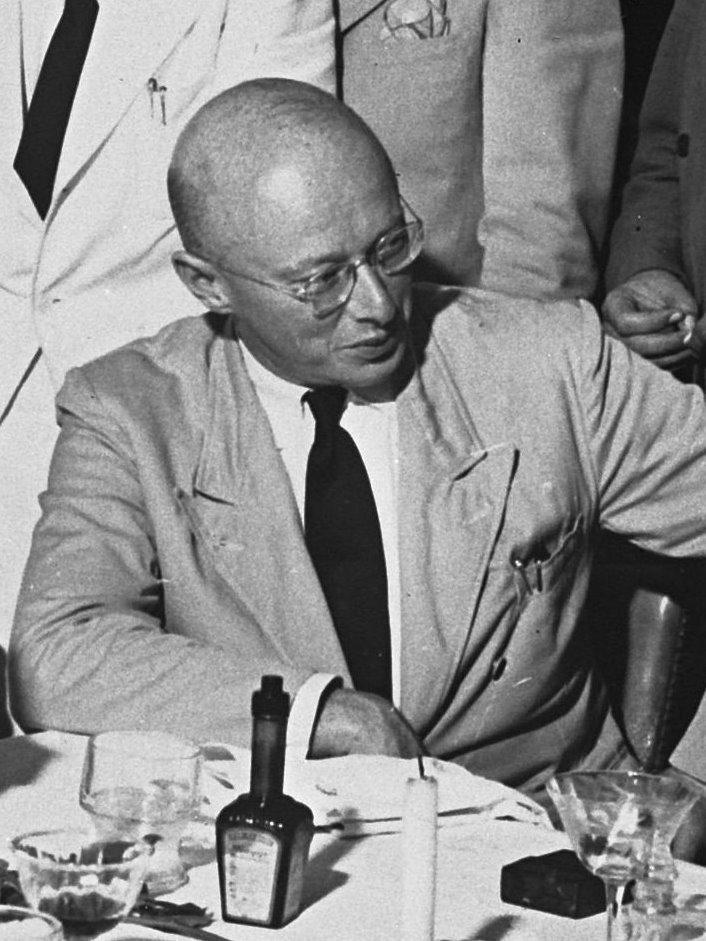
\includegraphics[width=1.5744in,height=2.1016in]{Kurzbiographien-img027.jpg}}
\end{figure}
Anfang 1943 inhaftiert, wurde er mit seiner Frau Albertine Sophie (Tineke) van Raalte und seinen drei Kindern 3 am
22.04.43 mit dem Transport Transport XXIV/1 in das Ghetto Theresienstadt deportiert. Dort wurde er Mitglied der
Werkstatt für angewandte Kunst und Gemälde, später Atelier Spier genannt. Aus seinen Arbeiten in dieser Zeit wurde das
offizielle für Propagandazwecke in Auftrag gegebene, Andenkenalbum \textit{Bilder aus Theresienstadt} zusammengestellt.
Für den Propagandafilm, in welchem er selbst als Zuhörer bei der Choraufführung in der \textit{Titelszene }(1 bei
0:27min) auftritt, erstellte Jo Spier eine einzigartige Zeichendokumentation der Drehtage. Er wurde mit seiner Familie
am späten Abend des 08.05.1945 in Theresienstadt durch die Rote Armee befreit. Er kehrte zurück in die Niederlande,
wanderte aber wegen eines nicht nachgewiesenen Vorwurfs der Kollaboration 1951 in USA aus, wo er seinen Beruf als
Illustrator erfolgreich wieder aufnehmen konnte.


\bigskip

\textbf{Eigene Werke:}

\begin{itemize}
\item The Creation, text from Genesis, hand-lettered by Joseph P Ascherl, New York: Doubleday \& Company, 1970. 
\item  The Squirrel and the Harp, by David DeJong, New York: Macmillan, 1966.  
\item The Spice Cookbook, by Avanelle Day and Lillie Stuckey, David White Company, 1964  
\item Waters of the New World: Houston to Nantucket, by Jan de Hartog, New York: Atheneum, 1961.  
\item Peter Stuyvesant of Old New York, by Anna Crouse and Russel Crouse, New York: Random House, 1954.  
\item The Story of Louis Pasteur, by Alida Sims Malkus, New York: Grosset \& Dunlap, 1952.  
\item One Sky to Share: The French and American Journals of Raymond Leopold Bruckberger, New York: P. J. Kenedy \& Sons,
1952.  
\item Holland's House: a Nation Building a Home, by Peter Bricklayer, Haarlem, Netherlands: Joh. Enschede En Zonen,
1939.  
\item Mijn Jordanertjes : kinderen, die ik gekend heb, by A van Vlaardingen, Utrecht: Bijleveld, 1931. 
\item Godfried Bomans: Kopstukken. Ill. Jo Spier. Amsterdam, Brussel, Elsevier 1947 etc. (27th pr., 1987)
\end{itemize}

\bigskip

\textbf{Sekundärliteratur:}

\begin{itemize}
\item Peter van Straaten \& Jo Spier. Virtuoze tekenaars van het Nederlandse leven. Persmuseum Amsterdam, 2012.  
\item Jo Spier. Tekenaar van een tijdperk Samenst. door G.E. van Baarsel. Stedelijk Museum Zutphen, 2000. ISBN
90-805756-1-5  
\item Jo Spier: Album. Amsterdam, Elsevier, 1957. 
\item Michel van der Plas: Vader en moeder. Baarn, Bosch\& Keuning, 1987. ISBN 90-246-4621-9 (Interviews with children
of famous parents, a.o. Peter Spier) 
\item Eva Strusková, Jana Šplíchalová, Tomáš Fedorovič, Václav Kofroň: Wahrheit und Lüge. Dreharbeiten im Ghetto
Theresienstadt 1942–1945. Jüdisches Museum in Prag \& Nationalfilmarchiv (Hsg.). 2013.
\end{itemize}

\bigskip


\bigskip

\textbf{Internetquellen:}

\begin{itemize}
\item \url{http://www.ghetto-theresienstadt.de/pages/s/spierj.htm} 
\item \url{https://www.lambiek.net/artists/s/spier_j.htm} 
\item \url{https://en.wikipedia.org/wiki/Jo_Spier} 
\end{itemize}

\bigskip

\textbf{Bildquelle:}

\begin{itemize}
\item \url{https://www.wikidata.org/wiki/Q2683316} 
\end{itemize}
\textbf{Prof. Dr. Emil Utitz} [geb. 27.05.1883 in Roztoky (Böhmen); gest. 02.11.1956 in Jena (Bundesrepublik
Deutschland)] war ein tschechisch-deutschsprachiger Philosoph, Psychologe und Kunsttheoretiker.

\begin{figure}[h]
\centering
\lfbox[margin-top=0.1181in,margin-right=0.1181in,margin-bottom=0.1181in,margin-left=0.1181in,border-style=none,padding=0mm,vertical-align=top,raise=-0.9055in]{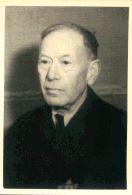
\includegraphics[width=1.5744in,height=2.3264in]{Kurzbiographien-img028.jpg}}
\end{figure}
Bis 1916 Privatdozent für Philosophie. 1919 Lehrauftrag für Ästhetik und Psychologie an der Universität Rostock. Dort
auch 1921-1924 Professor für Philosophie. 1925-1933 Professor an der Friedrichs-Universität Halle. Am 29.04.1933 durch
die Nationalsozialisten vorläufig beurlaubt. Am 23.09.1942 in den endgültigen Ruhestand versetzt. Emigration nach Prag.
Dort Lehrstuhlinhaber für Philosophie an der deutschen Karl-Ferdinands-Universität. 

Er wurde mit seiner Frau Ottilie (geb. Schwarzkopf) am 30.07.42 mit dem Transport Aav-268 in das Ghetto Theresienstadt
deportiert. Im Ghetto war er Leiter der \textit{Ghettozentralbücherei}. Zeitweilig war er stellvertretender Leiter der
\textit{Freizeitgestaltung}. Utitz und Baeck hielten in Theresienstadt umfangreiche Vorträge zu verschiedenen Themen.
Utitz hielt seinen ersten Vortrag am 24.11.1942 über die seelische Hygiene in Theresienstadt. Im Propoganadafilm ist er
als Vortragender in der Sequenz Vortrag (33) zu ehen. Er wurde am späten Abend des 08.05.1945 in Theresienstadt durch
die Rote Armee befreit. 


\bigskip

\textbf{Eigene Werke (Auswahl):}

\begin{itemize}
\item Grundlegung der allgemeinen Kunstwissenschaft. 2 Bände. Verlag Ferdinand Enke. Stuttgart 1914–1920.  
\item Die Gegenständlichkeit des Kunstwerks. Als: Philosophische Vorträge. Band 17. Verlag Reuther \& Reichard. Berlin
1917. .  
\item Die Kultur der Gegenwart in den Grundzügen dargestellt. Verlag Ferdinand Enke. Stuttgart 1921.  
\item Der Künstler. Vier Vorträge. Verlag Ferdinand Enke. Stuttgart 1925.  
\item Lehrbuch der Philosophie. Herausgegeben von Max Dessoir. Band 2: Die Philosophie in ihren Einzelgebieten.
Dargestellt von Erich Becher: Erkenntnistheorie und Metaphysik. Kurt Koffka: Psychologie. Paul Menzer: Ethik. Johann
Baptist Rieffert: Logik. Moritz Schlick: Naturphilosophie. Paul Tillich: Religionsphilosophie. Emil Utitz: Ästhetik und
Philosophie der Kunst. Berlin 1925.  
\item Die Überwindung des Expressionismus. Charakterologische Studien zur Kultur der Gegenwart. Verlag Ferdinand Enke.
Stuttgart 1927.  
\item Mensch und Kultur. Verlag Ferdinand Enke. Stuttgart 1933.  
\item Die Sendung der Philosophie in unserer Zeit. Verlag Sijthoff. Leiden (Niederlande) 1935.  
\item Masaryk als Volkserzieher. Festvortrag aus Anlass des 85. Geburtstages Tomáš Garrigue Masaryk. Prag 1935.  
\item Psychologie zivota Terezinskem koncentracznim tabore. Prag 1947  
\item Psychologie des Lebens im Konzentrationslager Theresienstadt. Verlag A. Sexl. Wien 1948.  
\item Egon Erwin Kisch. Der klassische Journalist. Aufbau-Verlag. Berlin 1956.  
\end{itemize}

\bigskip

\textbf{Sekundärliteratur:}

\begin{itemize}
\item Georg Mende: Emil Utitz zum Gedenken; in: Wissenschaftliche Zeitschrift der Friedrich-Schiller-Universität Jena
(Gesellschafts- und sprachwissenschaftliche Reihe) 6(1956/57)1/2, S. 1–2.  
\item Heinz Grassel: Zur Entwicklung der Psychologie an der Universität Rostock; in: Wissenschaftliche Zeitschrift der
Wilhelm-Pieck-Universität Rostock (Gesellschafts- und Sprachwissenschaftliche Reihe) 20(1971)3/4, S. 155–163. 
\item  Anna Hyndráková, Helena Krejčová, Jana Svobodová: Prominenti v ghettu Terezín 1942–1945. Dokumenty. Ústav pro
soudobé dějiny AV ČR, Prag 1996.  
\item Henrik Eberle: Die Martin-Luther-Universität in der Zeit des Nationalsozialismus. Mitteldeutscher Verlag, Halle
2002, ISBN 3-89812-150-X, S. 394f  
\item Reinhard Mehring: Das Konzentrationslager als ethische Erfahrung. Zur Charakterologie von Emil Utitz. In: Deutsche
Zeitschrift für Philosophie. Band 51. 2003. S. 761–775.  
\item Reinhard Mehring (Hrsg.): Ethik nach Theresienstadt. Späte Texte des Prager Philosophen Emil Utitz (1883–1956).
Königshausen \& Neumann, Würzburg 2015, ISBN 978-3-8260-5655-0.  
\item Reinhard Mehring: Philosophie im Exil. Emil Utitz, Arthur Liebert und die Exilzeitschrift Philosophia.
Dokumentation zum Schicksal zweier Holocaust-Opfer. Königshausen \& Neumann, Würzburg 2018, ISBN 978-3-8260-6449-4.  
\item Uwe Wolfradt: Emil Utitz (1883–1956) – Ein Psychologe berichtet aus dem Lager Theresienstadt. In: Martin Wieser
(Hg.): Psychologie im Nationalsozialismus, Berlin u. a.: Peter Lang 2020 (Beiträge zur Geschichte der Psychologie; 32),
ISBN 978-3-631-80392-9, S. 89–104.
\end{itemize}

\bigskip

\textbf{Internetquellen:}

\begin{itemize}
\item \url{http://www.ghetto-theresienstadt.de/pages/u/utitze.htm} 
\item \url{https://de.wikipedia.org/wiki/Emil_Utitz} 
\end{itemize}

\bigskip

\textbf{Bildquelle:}

\begin{itemize}
\item \url{http://www.ghetto-theresienstadt.de/images/prominente/Bild9.gif} 
\end{itemize}
\textbf{Ellie Marie Friederike Julie von Bleichröder }[geb. 17.09.1894 in Drehsa (Deutsches Reich); gest. 1989] war die
Tochter von James und Harriet von Bleichröder. 

\begin{figure}[h]
\centering
\lfbox[margin-top=0.1181in,margin-right=0.1181in,margin-bottom=0.1181in,margin-left=0.1181in,border-style=none,padding=0mm,vertical-align=top,raise=-0.9055in]{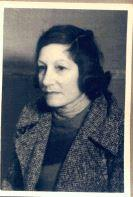
\includegraphics[width=1.5744in,height=2.3299in]{Kurzbiographien-img029.jpg}}
\end{figure}
Am 9. Dezember 1916 heiratete sie den Kaufmann Rudolph Alfred Herrschel. Dieser war Inhaber der Rohtabakgroßhandlung
Rudolph A. Herrschel. In den 1950er Jahren Kommanditistin des Münchner Bankhauses Neuvians, Reuschel \& Co. Sie wurde
am 27.07.1942 mit dem Transport 1/31–2364 in das Ghetto Theresienstadt deportiert.Ihre Rolle im Ghetto ist unebkannt.
Im Propoganadafilm ist sie in den Sequenzen 22 23 Propagandafilms Theresienstadt zu sehen. Sie sitzt während des
\textit{Vortrages }von Utitz in der zweiten Reihe und ist als einzige junge Frau deutlich zu erkennen (33 bei 18:51min
). Sie wurde am späten Abend des 08.05.1945 in Theresienstadt durch die Rote Armee befreit.


\bigskip

\textbf{Eigene Werke:}

\begin{itemize}
\item \url{https://archives.cjh.org//repositories/5/resources/6774} 
\end{itemize}

\bigskip

\textbf{Internetquellen:}

\begin{itemize}
\item \url{http://www.ghetto-theresienstadt.de/pages/b/bleichroedere.htm} 
\item \url{https://de.wikipedia.org/wiki/Ellie_von_Bleichr%C3%B6der#cite_note-2} 
\end{itemize}

\bigskip

\textbf{Bildquelle:}

\begin{itemize}
\item \url{http://www.ghetto-theresienstadt.de/images/prominente/Bild118.gif} 
\end{itemize}
\textbf{Clara von Schultz} (geb. Petite) [geb. 08.07.1862 in St. Thomas (Westindien); gest. 1963], Dänin, war die
Ehefrau von Johann Hermann (von) Schultz, der Flotten-Kommandeur der dänischen Flotte war. 

\begin{figure}[h]
\centering
\lfbox[margin-top=0.1181in,margin-right=0.1181in,margin-bottom=0.1181in,margin-left=0.1181in,border-style=none,padding=0mm,vertical-align=top,raise=-0.9055in]{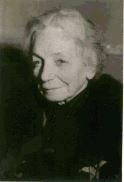
\includegraphics[width=1.5744in,height=2.3146in]{Kurzbiographien-img030.jpg}}
\end{figure}
Sie wurden am 05.10.1943 in das Ghetto Theresienstadt deportiert. Ihre Rolle im Ghetto ist unbekannt. Im Propoganadafilm
ist sie in der Sequenz \textit{Terrasse} (4) zu sehen. Sie wurde am späten Abend des 08.05.1945 in Theresienstadt durch
die Rote Armee befreit.


\bigskip

\textbf{Internetquellen:}

\begin{itemize}
\item \url{http://www.ghetto-theresienstadt.de/pages/s/schultzc.htm} 
\item \url{https://collections.ushmm.org/search/catalog/pa1144027} 
\end{itemize}

\bigskip


\bigskip

\textbf{Bildquelle:}

\begin{itemize}
\item \url{http://www.ghetto-theresienstadt.de/images/prominente/Bild30.gif} 
\end{itemize}
\textbf{Julie Salinger} (auch Julia Frieda Ziemann/Zeman) [geb. 06.06.1873 in Sárvár (Österreich-Ungarn); gest.
12.04.1947 in Berlin-Wedding (West-Berlin)] war ein ungarisch-deutsche Opern- und Kammersängerin (Sopran) aus Hamburg. 

\begin{figure}[h]
\centering
\lfbox[margin-top=0.1181in,margin-right=0.1181in,margin-bottom=0.1181in,margin-left=0.1181in,border-style=none,padding=0mm,vertical-align=top,raise=-0.9055in]{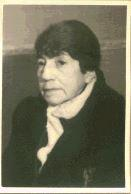
\includegraphics[width=1.5744in,height=2.3264in]{Kurzbiographien-img031.jpg}}
\end{figure}
1894-1933 als Opernsängerin vor allem in Hamburg tätig und wurde als Königlich-preußische Kammersängerin ausgezeichnet.
Zwei uneheliche Söhne mit Prinz Heinrich von Preußen, Bruder des deutschen Kaisers Wilhelm II. Im Ersten Weltkriegs
Lazarettschwester. 

Sie wurde am 17.06.1942 mit dem Transport 1896–1/26 in das Ghetto Theresienstadt deportiert. Ihre Rolle im Ghetto ist
unbekannt. Im Propoganadafilm ist sie in der Sequenz \textit{???} (8 bei 3.50min) zu sehen. Sie wurde am späten Abend
des 08.05.1945 in Theresienstadt durch die Rote Armee befreit.


\bigskip

\textbf{Sekundärliteratur:}

\begin{itemize}
\item Kay Weniger: Zwischen Bühne und Baracke. Lexikon der verfolgten Theater-, Film- und Musikkünstler 1933 bis 1945.
Metropol, Berlin 2008, ISBN 978-3-938690-10-9, S. 410 
\item  Karel Magry: „Das Konzentrationslager als Idylle: {\textquotedbl}Theresienstadt{\textquotedbl} – Ein
Dokumentarfilm aus dem jüdischen Siedlungsgebiet“. In: Fritz-Bauer-Institut (Hg.): Auschwitz : Geschichte, Rezeption
und Wirkung. Frankfurt : Campus, 1997, S. 319–352, hier S. 338
\item Karel Magry: Das Konzentrationslager als Idylle: „Theresienstadt“ – Ein Dokumentarfilm aus dem jüdischen
Siedlungsgebiet. In: Fritz-Bauer-Institut (Hrsg.): Auschwitz – Geschichte, Rezeption und Wirkung. Campus, Frankfurt
1997, S. 319–352, hier S. 338.
\end{itemize}

\bigskip

\textbf{Internetquellen:}

\begin{itemize}
\item \url{http://www.ghetto-theresienstadt.de/pages/s/salingerj.htm} 
\item \url{https://de.wikipedia.org/wiki/Julie_Salinger_(S%C3%A4ngerin}) 
\end{itemize}

\bigskip

\textbf{Bildquelle:}

\begin{itemize}
\item \url{http://www.ghetto-theresienstadt.de/images/prominente/Bild34.gif} 
\end{itemize}
\textbf{Dr. Benjamin Murmelstein }[geb. 09.06.1905 in Lemberg (Österreich-Ungarn (Galizien)); gest. 27.10.1989 in Rom
(Italien)] war ein österreichischer Rabbiner, Gelehrter und Funktionär der Israelitischen Kultusgemeinde Wien.

\begin{figure}[h]
\centering
\lfbox[margin-top=0.1181in,margin-right=0.1181in,margin-bottom=0.1181in,margin-left=0.1181in,border-style=none,padding=0mm,vertical-align=top,raise=-0.9055in]{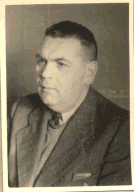
\includegraphics[width=1.5744in,height=2.2516in]{Kurzbiographien-img032.png}}
\end{figure}
Nach dem Anschluss Österreichs im März 1938 war er Leitungsmitglied der Israelitischen Kultusgemeinde Wien. Er leitete
später die vom NS-Regime geschaffene \textit{Auswanderungsabteilung} in der Wiener Kultusgemeinde. Er musste dabei eng
mit \textit{Zentralstelle für jüdische Auswanderung in Wien} kooperieren, die einzig dem Ziel diente, die Emigration
von Wiener Juden zu forcieren. In dieser Funktion konnte er vielen jüdischen Wienern das Leben retten. Bis November
1941 konnten etwa 128.000 Juden aus Wien emigrieren. Ab 1942 musste er mit anderen jüdischen Funktionären während der
Abfertigung der Deportationszüge aus Wien in die Vernichtungslager im Osten auf Weisung der NS-Behörden die
\textit{Einwaggonierung} vornehmen, was nicht zu verhindern war. Ab November 1942 war er im Beirat des Ältestenrates
der Juden in Wien unter dessen Leiter Löwenherz. Er wurde mit seiner Frau Margit (geb. Geyer) und seinem Sohn Wolf
Murmelstein (geb. 1936) am 29.01.43 in das Ghetto Theresienstadt deportiert. Im Ghetto war er Zweiter Stellvertreter
des Judenältesten Paul Eppsteins. Ab 27.09.44 Judenältester. Im Propoganadafilm ist er in der während einer Besprechung
des Ältestenrates rechts neben Eppstein in der Sequenz \textit{Vortrag} (10 bei 4:36min) zu sehen. Er wurde am späten
Abend des 08.05.1945 in Theresienstadt durch die Rote Armee befreit. Nach Kriegsende blieb er in Theresienstadt und
wirkte bei der Auflösung des Ghettos mit und verfasste dort noch im Mai/Juni 1945 seine Zeitzeugenberichte. Danach
wanderte wegen Kollaboration angefeindet nach Italien aus. 


\bigskip

\textbf{Eigene Werke:}

\begin{itemize}
\item Benjamin Murmelstein: Theresienstadt Eichmanns Vorzeige-Ghetto. Mit einem Nachwort von Wolf Murmelstein. Deutsche
Übersetzung der 1961 in Italienisch erschienenen Autobiographie Terezin. Il ghetto-modello di Eichmann. Wien 2014, ISBN
978-3-7076-0510-5.  
\item Terezin. Il ghetto-modello di Eichmann. Cappelli, Bologna 1961 (2. Auflage, La Scuola, Milano 2013, mit Nachwort
von Wolf Murmelstein: Benjamin Murmelstein, „Il testimone mai sentito“. S. 237–246).  
\item Geschichte der Juden. Des Volkes Weltwandern. Josef Belf, Wien 1938.  Adam. Ein Beitrag zur Messiaslehre. Diss.
Universität Wien 1927.
\end{itemize}

\bigskip

\textbf{Sekundärliteratur:}

\begin{itemize}
\item Eva Strusková, Jana Šplíchalová, Tomáš Fedorovič, Václav Kofroň: Wahrheit und Lüge. Dreharbeiten im Ghetto
Theresienstadt 1942–1945. Jüdisches Museum in Prag \& Nationalfilmarchiv (Hsg.). 2013.  
\item Hans Günther Adler: Theresienstadt 1941–1945. Das Antlitz einer Zwangsgemeinschaft. Geschichte, Soziologie,
Psychologie. Mohr (Siebeck), Tübingen 1955 (2., verbesserte und ergänzte Auflage, ebenda 1960; Reprint der Ausgabe 1960
mit einem Nachwort von Jeremy Adler, Wallstein-Verlag, Göttingen 2005, ISBN 3-89244-694-6).  
\item Anna Hájková: Der Judenälteste und seine SS-Männer. Benjamin Murmelstein und seine Beziehung zu Adolf Eichmann und
Karl Rahm. In: Ronny Loewy, Katharina Rauschenberger (Hrsg.): „Der Letzte der Ungerechten“: der „Judenälteste“ Benjamin
Murmelstein in Filmen 1942–1975. Frankfurt am Main/New York 2011.  
\item Herbert Rosenkranz: Verfolgung und Selbstbehauptung: die Juden in Österreich 1938–1945. Herold, Wien 1978, ISBN
3-7008-0150-5.  
\item Doron Rabinovici: Instanzen der Ohnmacht. Wien 1938–1945. Der Weg zum Judenrat. Jüdischer Verlag, Frankfurt 2000,
ISBN 3-633-54162-4.  
\item Axel Feuß: Das Theresienstadt-Konvolut. Dölling und Galitz, Hamburg u. a. 2002, ISBN 3-935549-22-9.  
\item Ronny Loewy, Katharina Rauschenberger (Hrsg.): „Der Letzte der Ungerechten“: der „Judenälteste“ Benjamin
Murmelstein in Filmen 1942–1975. Wissenschaftliche Reihe des Fritz-Bauer-Instituts, Bd. 19, Campus Verlag, Frankfurt am
Main/New York 2011, ISBN 978-3-593-39491-6.  
\item Marc Zitzmann: Der letzte „Judenälteste“ – Retter oder Verräter? In: Neue Zürcher Zeitung. 10. Dezember 2013.
\item Elfstündiges Interview Lanzmanns mit Murmelstein über seine Funktion in Wien und Theresienstadt von 1938 bis 1945
beim Steven Spielberg Film and Video Archive des United States Holocaust Memorial Museum (RG-60.5009, Tape 3158 -
3190). 
\end{itemize}

\bigskip


\bigskip

\textbf{Internetquellen:}

\begin{itemize}
\item \url{http://www.ghetto-theresienstadt.de/pages/m/murmelsteinb.htm} 
\item \url{https://de.wikipedia.org/wiki/Benjamin_Murmelstein} 
\end{itemize}

\bigskip

\textbf{Bildquelle:}

\begin{itemize}
\item \url{https://en.wikipedia.org/wiki/Benjamin_Murmelstein#/media/File:Benjamin_Murmelstein.gif} 
\end{itemize}
\textbf{Raphael Herz-Sommer }[geb. 21.06.1937; gest. 26.11.2001] war Sohn des Geigers Leopold Sommer und der Pianistin
Alice Herz-Sommer und (nach 1945) Cellist, Dirigent und Mitglied des Solomon Trio in London.

\begin{figure}[h]
\centering
\lfbox[margin-top=0.1181in,margin-right=0.1181in,margin-bottom=0.1181in,margin-left=0.1181in,border-style=none,padding=0mm,vertical-align=top,raise=-0.9055in]{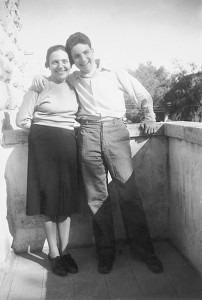
\includegraphics[width=1.5744in,height=2.3417in]{Kurzbiographien-img033.jpg}}
\end{figure}
Er wurden mit seinen Eltern am 1943 (genaues Datum unbekannt) in das Ghetto Theresienstadt deportiert. Im Ghetto spielt
den Spatz in der Kinderoper Brundibar. Er musste angeblich 50 mal eine der Hauptrollen in der Kinderoper übernehmen und
war am Ende nur eines der 130 überlebenden Kindern. Im Propoganadafilm ist er in der Sequenz \textit{Kinderoper} (17)
zu sehen. Er wurde am späten Abend des 08.05.1945 in Theresienstadt durch die Rote Armee befreit.


\bigskip

\textbf{Sekundärliteratur:}

\begin{itemize}
\item Christine Haiden: Vielleicht bin ich ja ein Wunder. Gespräche mit 100-Jährigen. Residenz, St. Pölten 2006, ISBN
3-7017-3023-7.  
\item Melissa Müller, Reinhard Piechocki: Alice Herz-Sommer – „Ein Garten Eden inmitten der Hölle“. Droemer, München
2006; Neuausgabe ebd. 2011, ISBN 978-3-426-78515-7.  
\item Caroline Stoessinger: Ich gebe die Hoffnung niemals auf: Hundert Jahre Weisheit aus dem Leben von Alice
Herz-Sommer. Mit einem Vorwort von Václav Havel (Originaltitel: A Century of Wisdom, übersetzt von Ralf Pannowitsch und
Christiane Wagler), Knaus, München 2012, ISBN 978-3-8135-0480-4.
\end{itemize}

\bigskip


\bigskip

\textbf{Internetquellen:}

\begin{itemize}
\item \url{https://interlude.hk/music-miracle-first-place-art-alice-herz-sommer/}
\item \url{https://de.wikipedia.org/wiki/Alice_Herz-Sommer}
\end{itemize}

\bigskip


\bigskip

\textbf{Bildquelle:}

\begin{itemize}
\item \url{https://interlude.hk/music-miracle-first-place-art-alice-herz-sommer/}
\end{itemize}
\textbf{Morits Oppenhejm} [geb. 01.04.1897 in Kopenhagen (Dänemark); gest. 05.07.1961 in Gentofte (Dänemark)] war ein
dänischer Rechtsberater der deutschen Botschaft in Kopenhagen.

\begin{figure}[h]
\centering
\lfbox[margin-top=0.1181in,margin-right=0.1181in,margin-bottom=0.1181in,margin-left=0.1181in,border-style=none,padding=0mm,vertical-align=top,raise=-0.9055in]{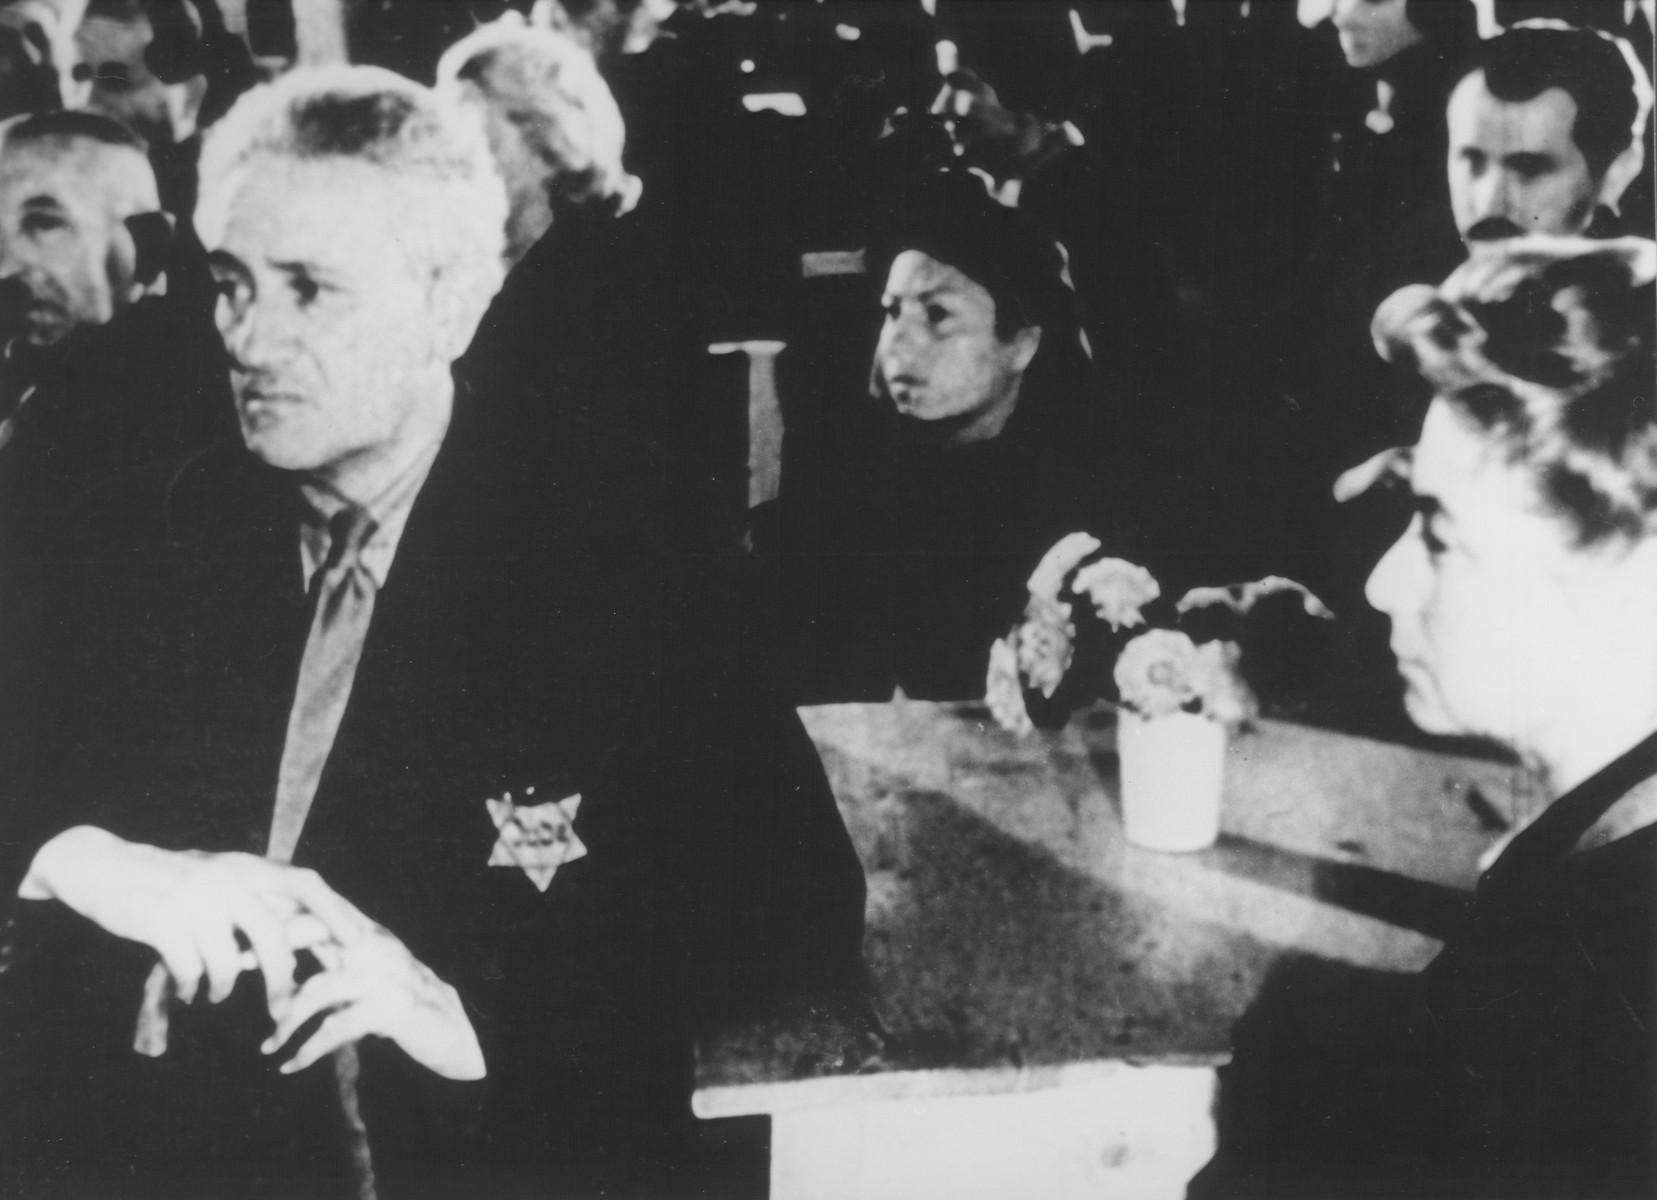
\includegraphics[width=1.5744in,height=1.1409in]{Kurzbiographien-img034.jpg}}
\end{figure}
Er wurde mit seiner Frau Mélanie (geb. Mathiason) und seinen Kindern Helmuth (geb. 1918), Ruth (geb. 1920), Ralph (geb.
1924) und Ellen (geb. 1926) am 13.10.1943 in das Ghetto Theresienstadt deportiert. Seine Rolle im Ghetto ist unbekannt.
Im Propagandafilm ist er in der Sequenz \textit{Konzert} (34 bei 19:32min) zu sehen. Mitte April 1945 wurde er im
Rahmen der Rettungsaktion der \textit{Weißen Busse} durch das Schwedische Rote Kreuz mit weiteren dänischen Häftlingen
aus Theresienstadt nach Schweden evakuiert.


\bigskip

\textbf{Bildquelle:}

\begin{itemize}
\item \url{https://collections.ushmm.org/search/catalog/pa1144050} 
\end{itemize}
\textbf{Mélanie Oppenhejm} (geb. Mathiason) [geb. 10.05.1897 in Hamburg (Deutsches Reich); gest. 03.12.1982 in Gentofte
(Dänemark)] war ein seit 1935 Vorsitzende der Jewish Women's Association in Kopenhagen. und ab 1940 Mitglied des
Präsidiums des dänischen Frauen-Zivildienstes.

\begin{figure}[h]
\centering
\lfbox[margin-top=0.1181in,margin-right=0.1181in,margin-bottom=0.1181in,margin-left=0.1181in,border-style=none,padding=0mm,vertical-align=top,raise=-0.9055in]{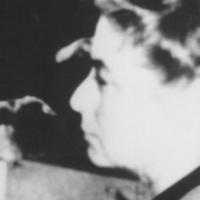
\includegraphics[width=1.5744in,height=1.5744in]{Kurzbiographien-img035.jpg}}
\end{figure}
Sie wurden mit ihrem Mann Morits Oppenhejm und ihren Kindern Helmuth (geb. 1918), Ruth (geb. 1920), Ralph (geb. 1924)
und Ellen (geb. 1926) am 13.10.1943 in das Ghetto Theresienstadt deportiert. Ihre Rolle im Ghetto ist unbekannt. Im
Propoganadafilm ist sie in der Sequenz beim \textit{Konzert} (34 bei 19:32min) zu sehen. Mitte April 1945 wurde er im
Rahmen der Rettungsaktion der \textit{Weißen Busse} durch das Schwedische Rote Kreuz mit weiteren dänischen Häftlingen
aus Theresienstadt nach Schweden evakuiert.


\bigskip

\textbf{Eigene Werke:}

\begin{itemize}
\item Theresienstadt : die Menschenfalle / Mélanie Oppenhejm ; aus dem Dänischen übersetzt von Dietmar Possart. URL:
https://collections.ushmm.org/search/catalog/bib44906 
\end{itemize}

\bigskip

\textbf{Internetquellen:}

\begin{itemize}
\item \url{https://www.kvinfo.dk/side/597/bio/895/%20Original%20Lin%20http://www.kvinfo.dk/side/597/bio/895/} 
\item \url{https://visualisations.ehri-project.eu/items/show/33} 
\end{itemize}

\bigskip


\bigskip

\textbf{Bildquelle:}

\begin{itemize}
\item https://visualisations.ehri-project.eu/items/show/33 ;
\url{https://collections.ushmm.org/search/catalog/pa1144050} 
\end{itemize}
\textbf{Ralph Oppenhejm} [geb. 10.12.1924 in Kopenhagen (Dänemark); gest. 04.02.2008 in Kopenhagen (Dänemark)], Sohn von
Morits und Mélanie Oppenhejm, war ein dänischer Schriftsteller (nach dem Krieg).

\begin{figure}[h]
\centering
\lfbox[margin-top=0.1181in,margin-right=0.1181in,margin-bottom=0.1181in,margin-left=0.1181in,border-style=none,padding=0mm,vertical-align=top,raise=-0.9055in]{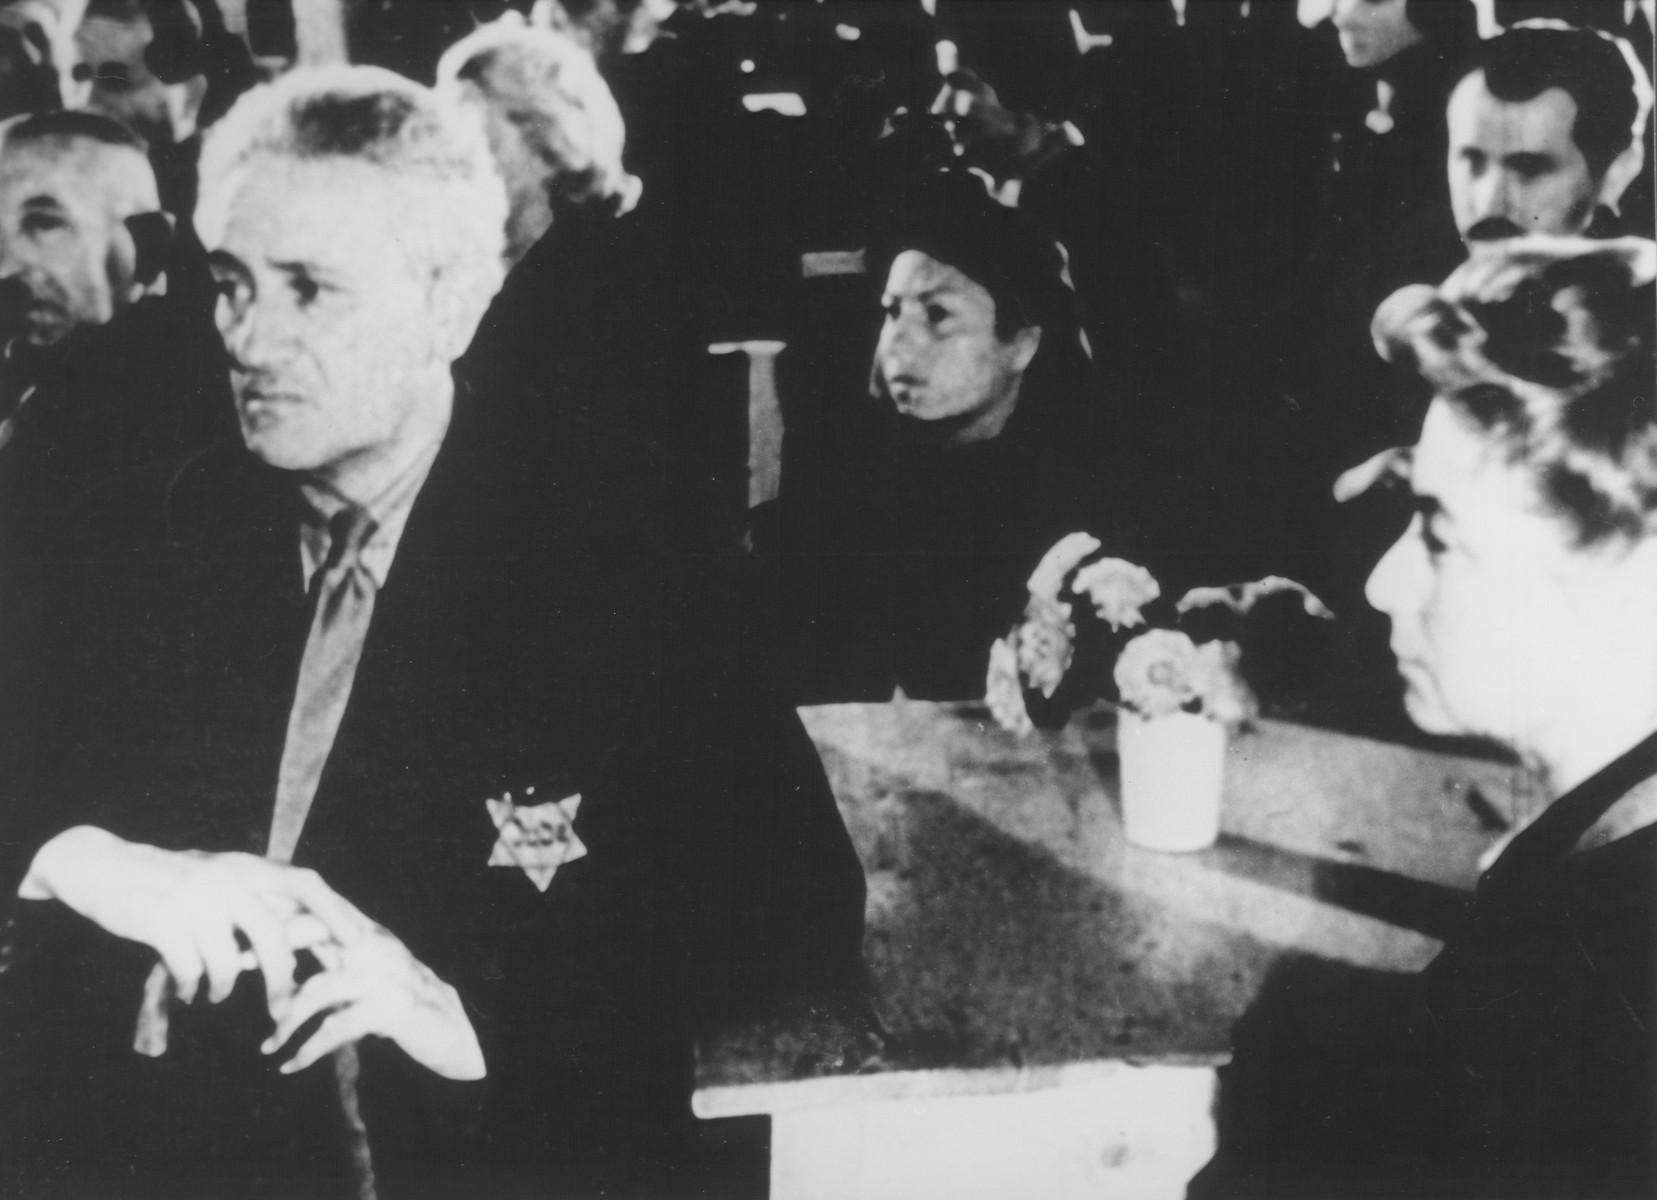
\includegraphics[width=1.5744in,height=1.1366in]{Kurzbiographien-img034.jpg}}
\end{figure}
Er wurden mit seiner Sohn von Morits und Mélanie Oppenhejm und seinen Geschwistern am 13.10.1943 in das Ghetto
Theresienstadt deportiert. Im Propagandafilm ist er in der Sequenz Konzert (34 bei 19:32min) als einziges Kind zu
sehen. Mitte April 1945 wurde er im Rahmen der Rettungsaktion der \textit{Weißen Busse} durch das Schwedische Rote
Kreuz mit weiteren dänischen Häftlingen aus Theresienstadt nach Schweden evakuiert.


\bigskip

\textbf{Internetquellen:}

\begin{itemize}
\item \url{http://www.ghetto-theresienstadt.de/pages/o/oppenhejmr.htm} 
\item \url{https://de.wikipedia.org/wiki/Ralph_Oppenhejm} 
\end{itemize}

\bigskip

\textbf{Bildquelle:}

\begin{itemize}
\item \url{https://collections.ushmm.org/search/catalog/pa1144050} 
\end{itemize}
\textbf{Phillip Kozower} [geb. 29.01.1894 in Berlin (Deutsches Reich); gest. nach 12.10.1944 (Deportation n. Auschwitz)
im KZ Auschwitz (Generalgouvernement Polen)] war ein deutscher Jurist und jüdischer Verbandsfunktionär bei der
Zionistischen Vereinigung für Deutschland (ZvfD) und der Jüdischen Volkspartei. 

\begin{figure}[h]
\centering
\lfbox[margin-top=0.1181in,margin-right=0.1181in,margin-bottom=0.1181in,margin-left=0.1181in,border-style=none,padding=0mm,vertical-align=top,raise=-0.9055in]{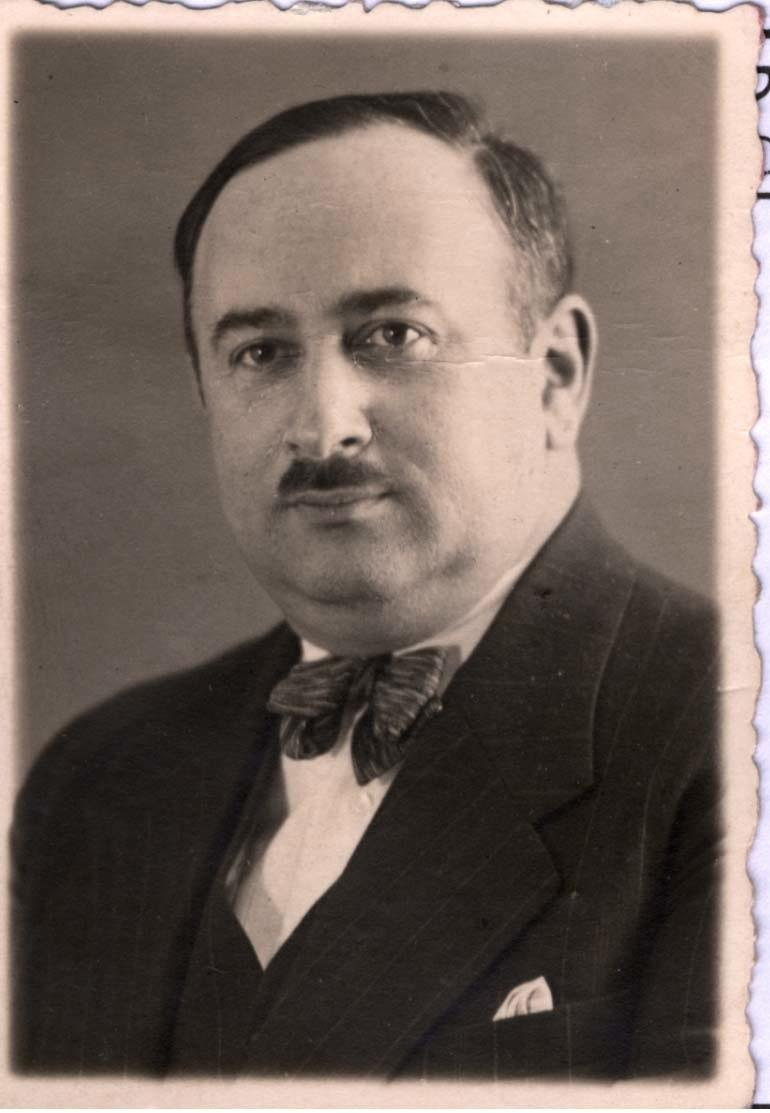
\includegraphics[width=1.5744in,height=2.2752in]{Kurzbiographien-img036.jpg}}
\end{figure}
1929-1943 gehörte er dem Vorstand der Jüdischen Gemeinde zu Berlin an, zuletzt als deren stellvertretender Vorsitzender.
Er wurden mit seiner Frau Gisela (geb. Herzberg) und seinen Kindern Eva Rita (geb. 20.05.1932), Alice (geb. 19.06.1934)
und Aron (geb. 13.11.1942) am 28.01.1943 mit dem Transport I / 87 in das Ghetto Theresienstadt deportiert. Im Ghetto
war er Mitglied im Ältestenrat, ab 15.04.1943 Leiter der Poststelle. Im Propoganadafilm ist er in der Sequenz
Abendessen (37) mit seiner Familie zu sehen, um so dem Zuschauer ein unbeschwertes Familienleben im Ghetto zu
suggerieren. Die Rolle der Großeltern mussten David Cohen und dessen Ehefrau übernehmen. Zugleich sieht man ihn auch in
der Sequenz Freilichtvarietee (22). Am 12.10.1944 wurde er mit seiner Familienach Auschwitz deportiert und dort
ermordet.


\bigskip

\textbf{Sekundärliteratur:}

\begin{itemize}
\item Otto Dov Kulka: Deutsches Judentum unter dem Nationalsozialismus, Band 1: Dokumente zur Geschichte der
Rechtsvertretung der deutschen Juden 1933–1939, Schriftenreihe wissenschaftlicher Abhandlungen des Leo Baeck Instituts
54, Mohr Siebeck, Tübingen 1997, ISBN 3-16-146413-3, S. 499.  
\item Susanne Krejsa: Spurensuche. Der NS-Anwalt und Judenretter Helmut Pfeiffer, Vergangenheitsverlag, Berlin 2011,
ISBN 3-864-08003-7, S. 110f, 148, 155, 157, 172.
\end{itemize}

\bigskip


\bigskip

\textbf{Internetquellen:}

\begin{itemize}
\item \url{http://www.ghetto-theresienstadt.de/pages/k/kozowerp.htm} 
\item \url{https://www.stolpersteine-berlin.de/de/biografie/342} 
\item \url{https://www.holocaust.cz/de/opferdatenbank/opfer/19590-philipp-kozower/} 
\item \url{https://de.wikipedia.org/wiki/Philipp_Kozower#cite_note-Nachama300-1}  
\end{itemize}

\bigskip

\textbf{Bildquelle:}

\begin{itemize}
\item \url{https://www.stolpersteine-berlin.de/de/biografie/342} 
\end{itemize}
\textbf{Else Schlitz, Gräfin von} (geb. Meyer) gen. von Götz [geb. 04.03.1882 in Kassel (Deutsches Reich); gest.
unbekannt] war die Ehefrau von Rudolf Graf von Schlitz, gen. von Görtz und von Wrisberg.

\begin{figure}[h]
\centering
\lfbox[margin-top=0.1181in,margin-right=0.1181in,margin-bottom=0.1181in,margin-left=0.1181in,border-style=none,padding=0mm,vertical-align=top,raise=-0.9055in]{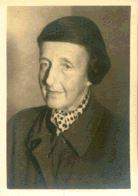
\includegraphics[width=1.5744in,height=2.2398in]{Kurzbiographien-img037.jpg}}
\end{figure}
Sie besuchte die Höhere Töchterschule, studierte dann Sprachen und Musik. Im 1. Weltkrieg leitete sie in Abwesenheit
ihres Gatten das Rittergut.

Sie wurdee mit ihrem Mann Rudolf Graf von Schlitz, gen. von Görtz und von Wrisberg und ihren drei Kindern am 07.04.1944
in das Ghetto Theresienstadt deportiert. Ihre Rolle im Ghetto ist unbekannt. Im Propoganadafilm ist sie in der Sequenz
\textit{Titelszene} (1 bei 0:26min) zu sehen. Sie wurde am späten Abend des 08.05.1945 in Theresienstadt durch die Rote
Armee befreit.


\bigskip

\textbf{Eigene Werke}:

\begin{itemize}
\item \url{https://shop.editionblaes.de/produkt/briefe-und-aufzeichnungen-von-else-graefin-von-schlitz/} 
\end{itemize}

\bigskip

\textbf{Internetquellen:}

\begin{itemize}
\item \url{http://www.ghetto-theresienstadt.de/pages/s/schlitze.htm} 
\end{itemize}

\bigskip

\textbf{Bildquelle:}

\begin{itemize}
\item \url{http://www.ghetto-theresienstadt.de/images/prominente/Bild32.gif} 
\end{itemize}
\textbf{Johann Friedländer} [geb. 05.11.1882 in Bern (Schweiz); gest. 20.01.1945 zwischen Auschwitz und Pless auf einem
der Todesmärsche (Generalgouvernement Polen)] war ein deutsch-österreichischer Feldmarschallleutnant des
österreichischen Bundesheeres.

\begin{figure}[h]
\centering
\lfbox[margin-top=0.1181in,margin-right=0.1181in,margin-bottom=0.1181in,margin-left=0.1181in,border-style=none,padding=0mm,vertical-align=top,raise=-0.9055in]{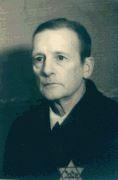
\includegraphics[width=1.5744in,height=2.4008in]{Kurzbiographien-img038.jpg}}
\end{figure}
Er wurden mit seiner Frau Leona Margarethe (geb. Abel) am 03.09.1943 mit dem Transport 936–IV/14 in das Ghetto
Theresienstadt deportiert. Seine Rolle im Ghetto ist unbekannt. Im Propoganadafilm ist er n der Sequenz
\textit{Terrasse} (4) zu sehen. Er wurde am 16. Oktober 1944 nach dem Tod seiner Frau Leona nach Birkenau zum
Arbeitseinsatz deportiert und 1945 auf dem Marsch von Auschwitz nach Pless von den Wachmannschaften erschossen.


\bigskip

\textbf{Sekundärliteratur:}

\begin{itemize}
\item Johann Friedländer, Offizier und NS-Opfer. In: Die Presse (Wien), 17. Jänner 1995.  
\item Martin Senekowitsch: Feldmarschalleutnant Johann Friedländer, 1882–1945. Ein vergessener Offizier des
Bundesheeres. Wien: BMLV, Büro für Wehrpolitik, 1995.
\end{itemize}

\bigskip

\textbf{Internetquellen:}

\begin{itemize}
\item \url{http://www.ghetto-theresienstadt.de/pages/f/friedlaenderj.htm} 
\item
\url{https://www.welt.de/welt_print/kultur/literatur/article5950928/Der-Feldmarschall-hat-zwei-Kugeln-bekommen.html} 
\item \url{https://de.wikipedia.org/wiki/Johann_Friedl%C3%A4nder} 
\end{itemize}

\bigskip

\textbf{Bildquelle:}

\begin{itemize}
\item \url{http://www.ghetto-theresienstadt.de/images/prominente/Bild99.gif} 
\end{itemize}
\textbf{Leon Neuberger} [geb. 24.04.1880 in Baince (Bezirk Sereth, Rumänien); gest. nach 12.10.1944 im KZ Auschwitz
(Generalgouvernement Polen)] war ein deutsch-österreichischer Berufsoffizier und hochdekorierter Frontkämpfer des
Ersten Weltkrieges.

\begin{figure}[h]
\centering
\lfbox[margin-top=0.1181in,margin-right=0.1181in,margin-bottom=0.1181in,margin-left=0.1181in,border-style=none,padding=0mm,vertical-align=top,raise=-0.9055in]{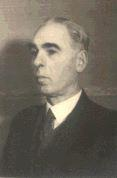
\includegraphics[width=1.5744in,height=2.3929in]{Kurzbiographien-img039.jpg}}
\end{figure}
Er wurden mit seiner Franziska (geb. Bielik) am 10.10.42 mit dem Transport 1292–IV/13 in das Ghetto Theresienstadt
deportiert. Im Ghetto war er der Leiter des \textit{Wach- und Ordnungsdienstes}. Im Propoganadafilm ist er in der
Sequenz Freilichtvarietee (22) zu sehen.


\bigskip

\textbf{Internetquellen:}

\begin{itemize}
\item \url{http://www.ghetto-theresienstadt.de/pages/n/neubergerl.htm} 
\end{itemize}
\begin{itemize}
\item \url{https://www.holocaust.cz/de/opferdatenbank/opfer/55606-leon-neuberger/}  
\end{itemize}

\bigskip

\textbf{Bildquelle:}

\begin{itemize}
\item \url{http://www.ghetto-theresienstadt.de/images/prominente/Bild52.gif} 
\end{itemize}
\textbf{Prof. Dr. Heinrich Adalbert Klang} [geb. 15.04.1875 in Wien (Österreich); gest. 22.01.1954 in Wien (Österreich)]
war ein deutsch-österreichischer Rechtswissenschaftler. Er war Professor für Bürgerliches Recht an der Universität Wien
und Senatspräsident am Obersten Gerichtshof in Wien.

\begin{figure}[h]
\centering
\lfbox[margin-top=0.1181in,margin-right=0.1181in,margin-bottom=0.1181in,margin-left=0.1181in,border-style=none,padding=0mm,vertical-align=top,raise=-0.9055in]{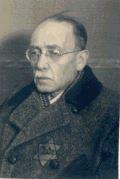
\includegraphics[width=1.5744in,height=2.3457in]{Kurzbiographien-img040.jpg}}
\end{figure}
Er wurden am 25.09.42 mit dem Transport 606–IV/11 in das Ghetto Theresienstadt deportiert. Im Ghetto war er Richter am
\textit{Ghettogericht}. Die Verhandlungsgegenstände am Ghettogericht der jüdischen Selbstverwaltung waren im
Wesentlichen Verlassenschaftsverfahren, Vormundschaften, Kuratelen und Strafrechtsangelegenheiten. Für die
österreichischen Häftlinge gehörte er dem Ältestenrat der jüdischen Selbstverwaltung in Theresienstadt an und
engagierte sich für seine Mitgefangenen. Im Propoganadafilm ist er in der Sequenz \textit{Bücherei} (32) zu sehen. Er
wurde am späten Abend des 08.05.1945 in Theresienstadt durch die Rote Armee befreit. Er heiratete 1952 die Witwe seines
Bruders Fritz. 


\bigskip

\textbf{Sekundärliteratur:}

\begin{itemize}
\item Heinrich Klang zum 75. Geburtstag. Festschrift herausgegeben in Verbindung mit der Juristischen Fakultät der
Universität Wien, der Österreichischen Richtervereinigung, der Rechtsanwaltskammer in Wien, Wien 1950 
\item Fritz Schwind: Klang, Heinrich. In: Neue Deutsche Biographie (NDB). Band 11, Duncker \& Humblot, Berlin 1977, ISBN
3-428-00192-3, S. 705 f. (Digitalisat). Felix Czeike (Hrsg.): Historisches Lexikon Wien. Band 3, Kremayr \& Scheriau,
Wien 1994, ISBN 3-218-00545-0, S. 522. 
\item Susanne Blumesberger, Michael Doppelhofer, Gabriele Mauthe: Handbuch österreichischer Autorinnen und Autoren
jüdischer Herkunft 18. bis 20. Jahrhundert. Band 2: J–R. Hrsg. von der Österreichischen Nationalbibliothek. Saur,
München 2002, ISBN 3-598-11545-8, S. 680. 
\item Johannes Feichtinger: Wissenschaft zwischen den Kulturen. Österreichische Hochschullehrer in der Emigration
1933–1945. Campus, Frankfurt am Main/New York 2001, ISBN 3-593-36584-7. 
\item Axel Feuß: Das Theresienstadt-Konvolut Altonaer Museum in Hamburg, Dölling und Galitz Verlag, Hamburg/München
2002, ISBN 3-935549-22-9. 
\item Günter Gößler, Martin Niklas: Heinrich Klang: Praxis und Theorie – Verfolgung und Rückkehr. In: Franz-Stefan
Meissel, Thomas Olechowski, Ilse Reiter-Zatloukal, Stefan Schima (Hrsg.): Vertriebenes Recht – Vertreibendes Recht. Zur
Geschichte der Wiener Rechts- und Staatswissenschaftlichen Fakultät zwischen 1938 und 1945 (= Juridicum Spotlight. Band
2). Manz, Wien 2012, ISBN 978-3-214-07405-0, S. 281–300.
\end{itemize}

\bigskip


\bigskip

\textbf{Internetquellen:}

\begin{itemize}
\item \url{http://www.ghetto-theresienstadt.de/pages/k/klangh.htm} 
\item \url{https://de.wikipedia.org/wiki/Heinrich_Klang} 
\end{itemize}

\bigskip

\textbf{Bildquelle:}

\begin{itemize}
\item \url{http://www.ghetto-theresienstadt.de/images/prominente/Bild75.gif} 
\end{itemize}
\textbf{Prof. Dr. Hermann Strauß} [geb. 28.04.1868 in Heilbronn (Deutsches Reich); gest. 17.10.1944 im Ghetto
Theresienstadt (Tschechoslowakei)] war ein deutscher Internist und Direktor der Abteilung für Innere Medizin des
Jüdischen Krankenhauses Berlin in der Zeit von 1910 bis 1942.

\begin{figure}[h]
\centering
\lfbox[margin-top=0.1181in,margin-right=0.1181in,margin-bottom=0.1181in,margin-left=0.1181in,border-style=none,padding=0mm,vertical-align=top,raise=-0.9055in]{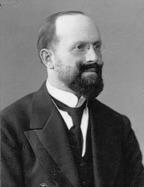
\includegraphics[width=1.5744in,height=2.0465in]{Kurzbiographien-img041.jpg}}
\end{figure}
Er wurden mit seiner Frau Elsa (geb. Isaac) und seine Sohn Walter (1900-1976) und einer weiteren Tochter am 31.07.1942
mit dem Transport I/35 in das Ghetto Theresienstadt deportiert. Im Ghetto gehörte Strauß ab Oktober 1942 dem
Ältestenrat an und war Leiter des \textit{wissenschaftlichen Ausschusses des Ghetto-Gesundheitswesens}. Im
Propoganadafilm ist er in der Sequenz \textit{Vortrag} (33) zu sehen.


\bigskip

\textbf{Eigene Werke:}

\begin{itemize}
\item Zur Technik des Aderlasses, der intravenösen und subcutanen Infusion. In: Zeitschrift für Krankenpflege. Bd. 20
(1898), H. 4, S. 66–69. 
\item Die chronischen Nierenentzündungen in ihrer Einwirkung auf die Blutflüssigkeit und deren Behandlung. Hirschwald,
Berlin 1902. 
\item Zur Behandlung und Verhütung der Nierenwassersucht. Therapie der Gegenwart 1903; N.F. 5: 193 - 200. 
\item Zur Methodik der Rectoskopie. Berlin Klin Wochenschr 1903; 40: 1100 - 1104. 
\item Vorlesungen über Diätbehandlung Innerer Krankheiten. Karger, Berlin 1910. 
\item Procto-Sigmoscopie und ihre Bedeutung für die Diagnostik und Therapie der Krankheiten des Rectums und der Flexura
sigmoidea. Thieme, Leipzig 1910. 
\item Erkrankungen des Rectum und Sigmoideum. Urban \& Schwarzenberg, Berlin/Wien 1922.
\end{itemize}

\bigskip

\textbf{Sekundärliteratur:}

\begin{itemize}
\item Helmut Schmolz, Hubert Weckbach: Bedeutende Heilbronner (III). In: Schwaben und Franken. Heimatgeschichtliche
Beilage der Heilbronner Stimme. 15. Jahrgang, Nr. 1, 11. Januar 1969, ZDB-ID 128017-X.  
\item Harro Jenss: Hermann Strauss. Internist und Wissenschaftler in der Charité und im jüdischen Krankenhaus Berlin (=
Jüdische Miniaturen. Bd. 95). Hentrich \& Hentrich, Berlin 2010, ISBN 978-3-941450-22-6.  
\item Harro Jenss: Von Heilbronn an die Charité und an das Jüdische Krankenhaus Berlin, Hermann Strauss 1868–1944. In:
Heilbronner Köpfe VI. Lebensbilder aus zwei Jahrhunderten (= Kleine Schriftenreihe des Archivs der Stadt Heilbronn. Bd.
58). Heilbronn 2011, S. 229–252.  
\item Harro Jenss, Peter Reinicke (Hrsg.): Der Arzt Hermann Strauss, 1868–1944. Autobiographische Notizen und
Aufzeichnungen aus dem Ghetto Theresienstadt. Hentrich \& Hentrich, Berlin 2014, ISBN 978-3-95565-048-3.  
\item Kilian Krauth: Der vergessene Mediziner aus der Klostergasse. Hermann Strauss machte in Berlin Karriere und endete
im KZ. In: Heilbronner Stimme. 25. Oktober 2014.  
\item Eberhard J. Wormer: Strauss, Hermann. In: Neue Deutsche Biographie (NDB). Band 25, Duncker \& Humblot, Berlin
2013, ISBN 978-3-428-11206-7, S. 511 f. (Digitalisat).  
\item Peter Reinicke: Strauss, Elsa, in: Hugo Maier (Hrsg.): Who is who der Sozialen Arbeit. Freiburg : Lambertus, 1998
ISBN 3-7841-1036-3, S. 581
\end{itemize}

\bigskip


\bigskip

\textbf{Internetquellen:}

\begin{itemize}
\item \url{http://www.ghetto-theresienstadt.de/pages/s/straussh.htm} 
\item \url{https://www.holocaust.cz/de/opferdatenbank/opfer/46922-hermann-strauss/} 
\item \url{https://de.wikipedia.org/wiki/Hermann_Strau%C3%9F_(Mediziner}) 
\end{itemize}

\bigskip

\textbf{Bildquelle:}

\begin{itemize}
\item
\href{https://upload.wikimedia.org/wikipedia/commons/5/5a/Hermann_Strau%C3%9F_(*_28._April_1868_in_Heilbronn%3B_%E2%80%A0_17._Oktober_1944_im_KZ_Theresienstadt).JPG}{https://upload.wikimedia.org/wikipedia/commons/5/5a/Hermann\_Strau\%C3\%9F\_\%28\%2A\_28.\_April\_1868\_in\_Heilbronn\%3B\_\%E2\%80\%A0\_17.\_Oktober\_1944\_im\_KZ\_Theresienstadt\%29.JPG} 
\end{itemize}
\textbf{Dr. Otto Stargardt} [geb. 25.07.1874 in Freienwalde a.d. Oder (Deutsches Reich); gest. unbekannt] war ein
deutscher Senatsmitglied des Reichsversorgungsgerichtes und Mitglied der evangelischen Provinzialsynode.

\begin{figure}[h]
\centering
\lfbox[margin-top=0.1181in,margin-right=0.1181in,margin-bottom=0.1181in,margin-left=0.1181in,border-style=none,padding=0mm,vertical-align=top,raise=-0.9055in]{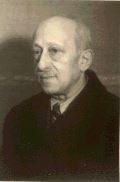
\includegraphics[width=1.5744in,height=2.3854in]{Kurzbiographien-img042.jpg}}
\end{figure}
Er wurden mit seiner Frau Edith (geb. Wolf) am 02.07.1942 mit dem Transport 798–I/14 in das Ghetto Theresienstadt
deportiert. Im Ghetto arbeitete er als \textit{Postzensor}. Im Propoganadafilm ist er zu sehen in der Sequenz
\textit{Vortrag} (33). Er wurde am späten Abend des 08.05.1945 in Theresienstadt durch die Rote Armee befreit. 


\bigskip

\textbf{Eigene Werke:}

\url{https://wiener.soutron.net/Portal/Default/en-GB/recordview/index/104727} 


\bigskip

\textbf{Internetquellen:}

\url{http://www.ghetto-theresienstadt.de/pages/s/stargardto.htm} 


\bigskip

\textbf{Bildquelle:}

\url{http://www.ghetto-theresienstadt.de/images/prominente/Bild22.gif} 

\textbf{Dr. Alexander Cohn} [geb. 04.09.1876 in Königsberg (Preußen); gest. 07.04.1951 in Berlin (Bundesrepublik
Deutschland)] war ein deutscher Kammergerichtsrat und dekorierter Frontkämpfer. 

\begin{figure}[h]
\centering
\lfbox[margin-top=0.1181in,margin-right=0.1181in,margin-bottom=0.1181in,margin-left=0.1181in,border-style=none,padding=0mm,vertical-align=top,raise=-0.8728in]{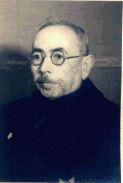
\includegraphics[width=1.5744in,height=2.3417in]{Kurzbiographien-img043.jpg}}
\end{figure}
Er war Autor juristischer Werke und gemeinsam mit Albert Mosse Mitarbeiter an einer Kommentierung des
Handelsgesetzbuches. Er wurden mit seiner Frau Else (geb. Hiller) am 28.01.1943 mit dem Transport 10723–I/87 in das
Ghetto Theresienstadt deportiert. Seine Rolle im Ghetto ist unbekannt. Im Propoganadafilm ist er in der Sequenz
\textit{Vortrag} (33) zu sehen. Er wurde am späten Abend des 08.05.1945 in Theresienstadt durch die Rote Armee befreit.



\bigskip

\textbf{Eigene Werke:}

\begin{itemize}
\item Herausgabe der Neuauflage Handelsgesetzbuch von Litthauer, 1905 (gemeinsam mit Albert Mosse)  
\item Auslieferungsverträge des Deutschen Reiches und der deutschen Einzelstaaten, 1908
\end{itemize}

\bigskip

\textbf{Sekundärliteratur:}

\begin{itemize}
\item Hans Bergemann/Simone Ladwig-Winters, Kammergericht (Hrsg.): Jüdische Richter am Kammergericht nach 1933 – Eine
Dokumentation, Verlag Carl Heymanns, 2004, ISBN 978-3-452-25833-5  
\item Axel Feuß: Das Theresienstadt-Konvolut, Altonaer Museum in Hamburg, Dölling und Galitz Verlag, Hamburg/München
2002, ISBN 3-935549-22-9
\end{itemize}

\bigskip


\bigskip

\textbf{Internetquellen:}

\begin{itemize}
\item \url{http://www.ghetto-theresienstadt.de/pages/c/cohna.htm} 
\item \url{https://de.wikipedia.org/wiki/Alexander_Cohn}  
\end{itemize}

\bigskip

\textbf{Bildquelle:}

\begin{itemize}
\item \url{http://www.ghetto-theresienstadt.de/images/prominente/Bild112.gif} 
\end{itemize}
\textbf{Prof. Dr. Arthur (Artur) Stein} [geb. 10.06.1871 in Wien (Österreich-Ungarn); gest. 15.11.1950 in Prag
(Tschechoslowakei)] war ein österreichisch-tschechischer Althistoriker und Universitätsprofessor in Prag.

\begin{figure}[h]
\centering
\lfbox[margin-top=0.1181in,margin-right=0.1181in,margin-bottom=0.1181in,margin-left=0.1181in,border-style=none,padding=0mm,vertical-align=top,raise=-0.9055in]{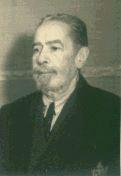
\includegraphics[width=1.5744in,height=2.2945in]{Kurzbiographien-img044.jpg}}
\end{figure}
Er wurden mit seiner Frau Flora (geb. Utitz) am 06.06.42 in das Ghetto Theresienstadt deportiert. Seine Rolle im Ghetto
ist unbekannt. Im Propoganadafilm ist er in der Sequenz \textit{Vortrag} (33) zu sehen. Er wurde am späten Abend des
08.05.1945 in Theresienstadt durch die Rote Armee befreit..


\bigskip

\textbf{Sekundärliteratur:}

\begin{itemize}
\item Artur Betz: Professor Arthur Stein gest.. In: Anzeiger für die Altertumswissenschaft. Band 4, 1951, Sp. 193 f.  
\item Martina Pesditschek: Stein, Arthur. In: Österreichisches Biographisches Lexikon 1815–1950 (ÖBL). Band 13, Verlag
der Österreichischen Akademie der Wissenschaften, Wien 2007–2010, ISBN 978-3-7001-6963-5, S. 146 f. (Direktlinks auf S.
146, S. 147).  
\item Volker Losemann: Stein, Arthur. In: Peter Kuhlmann, Helmuth Schneider (Hrsg.): Geschichte der
Altertumswissenschaften. Biographisches Lexikon (= Der Neue Pauly. Supplemente. Band 6). Metzler, Stuttgart/Weimar
2012, ISBN 978-3-476-02033-8, Sp. 1184–1186.
\end{itemize}

\bigskip

\textbf{Internetquellen:}

\begin{itemize}
\item \url{http://www.ghetto-theresienstadt.de/pages/s/steina.htm} 
\end{itemize}
\begin{itemize}
\item \url{https://de.wikipedia.org/wiki/Arthur_Stein_(Althistoriker}) 
\end{itemize}

\bigskip

\textbf{Bildquelle:}

\begin{itemize}
\item \url{http://www.ghetto-theresienstadt.de/images/prominente/Bild19.gif} 
\end{itemize}
\textbf{Prof. Dr. Leo Taussig} [geb. 01.12.1884 in Tlustitz bei Horschwitz (Böhmen); gest. nach 12.10.1944 im KZ
Auschwitz (Generalgouvernement Polen)] war ein bömischer außerordentlicher Professor für Psychologie und Neurologie und
mehrfach ausgezeichneter Offizier des Ersten Weltkrieges.

\begin{figure}[h]
\centering
\lfbox[margin-top=0.1181in,margin-right=0.1181in,margin-bottom=0.1181in,margin-left=0.1181in,border-style=none,padding=0mm,vertical-align=top,raise=-0.9055in]{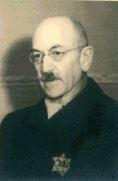
\includegraphics[width=1.5744in,height=2.4165in]{Kurzbiographien-img045.jpg}}
\end{figure}
Er wurde am 24.12.1942 mit dem Transport Ck in das Ghetto Theresienstadt deportiert. Im Ghetto war er Arzt in der
psychiatrischen Abteilung des Krankenhauses. Im Propoganadafilm ist er in der Sequenz \textit{Vortrag} (33) zu sehen.
Er wurde am 12.10.1944 in das KZ Auschwitz deportiert und dort ermordet.


\bigskip


\bigskip

\textbf{Internetquellen:}

\begin{itemize}
\item \url{http://www.ghetto-theresienstadt.de/pages/p/protektorat.htm} 
\item \url{https://www.holocaust.cz/de/opferdatenbank/opfer/129431-leo-taussig/} 
\end{itemize}

\bigskip

\textbf{Bildquelle:}

\begin{itemize}
\item \url{http://www.ghetto-theresienstadt.de/images/prominente/Bild15.gif} 
\end{itemize}
\textbf{Dr. Ernst Rosenthal} [geb. unbekannt ; gest. unbekannt] war 1933 Geschäftsführer des \textit{Reichsbundes
jüdischer Frontsoldaten und }Mitglied des KC (Kartell Convent deutscher Studenten jüdischen Glaubens).

Im Ghetto war erLeiter der \textit{Detektivabteilung}. Im Propoganadafilm ist er zu sehen in der Sequenz
\textit{Konzert} (34). Er wurde am späten Abend des 08.05.1945 in Theresienstadt durch die Rote Armee.


\bigskip


\bigskip

\textbf{Internetquellen:}

\begin{itemize}
\item \url{http://www.ghetto-theresienstadt.de/pages/r/rosenthale.htm} 
\item \url{https://portal.ehri-project.eu/units/us-005571-78012} 
\end{itemize}

\bigskip

\textbf{Dr. Erich Springer} [geb. unbekannt; gest. nach 1945] war ein Arzt.

Im Ghetto war er Leiter der Chirurgie im Ghetto. Im Propoganadafilm ist er zu sehen in der Sequenz \textit{Konzert}
(34). Er wurde (vermutlich) am späten Abend des 08.05.1945 in Theresienstadt durch die Rote Armee befreit.


\bigskip


\bigskip

\textbf{Sekundärliteratur:}

\begin{itemize}
\item
\url{https://books.google.de/books?id=yh-_DwAAQBAJ&pg=PT30&lpg=PT30&dq=springer+erich+theresienstadt&source=bl&ots=Fdj-ZD0MVN&sig=ACfU3U17FkWISPTY9yFD5jwgPakRrstsog&hl=de&sa=X&ved=2ahUKEwjgoZeK2aDtAhVPqaQKHa6WCOM4FBDoATABegQIAhAC#v=onepage&q=springer%20erich%20theresienstadt&f=false} 
\end{itemize}

\bigskip


\bigskip

\textbf{Internetquellen:}

\begin{itemize}
\item \url{https://portal.ehri-project.eu/units/il-002777-wp2_bt-053_000_000-053_000_067} 
\end{itemize}
\textbf{Prof. Dr. Alfred Klein} aus Jena bislang nichts zu dieser Person gefunden


\bigskip


\bigskip
\end{document}
